\section{Results}
In this section, we present the final results. Additionally, to these results,
we also provide tuning results that have guided our algorithm selection.

\subsection{F1}
Figure~\ref{fig:f1} shows the f1-scores for the six datasets.  We observe that
in the long run, the Mondrian algorithm with 5 or 10 trees achieves the best
f1-scores.  On most of the datasets (\banosdataset, \recofitdataset,
RandomTree) the best Mondrian is often followed by the HoeffdingTree and the
naïve Bayes classifiers. 

\begin{figure*}[ht]
	\begin{subfigure}[t]{.5\linewidth}
		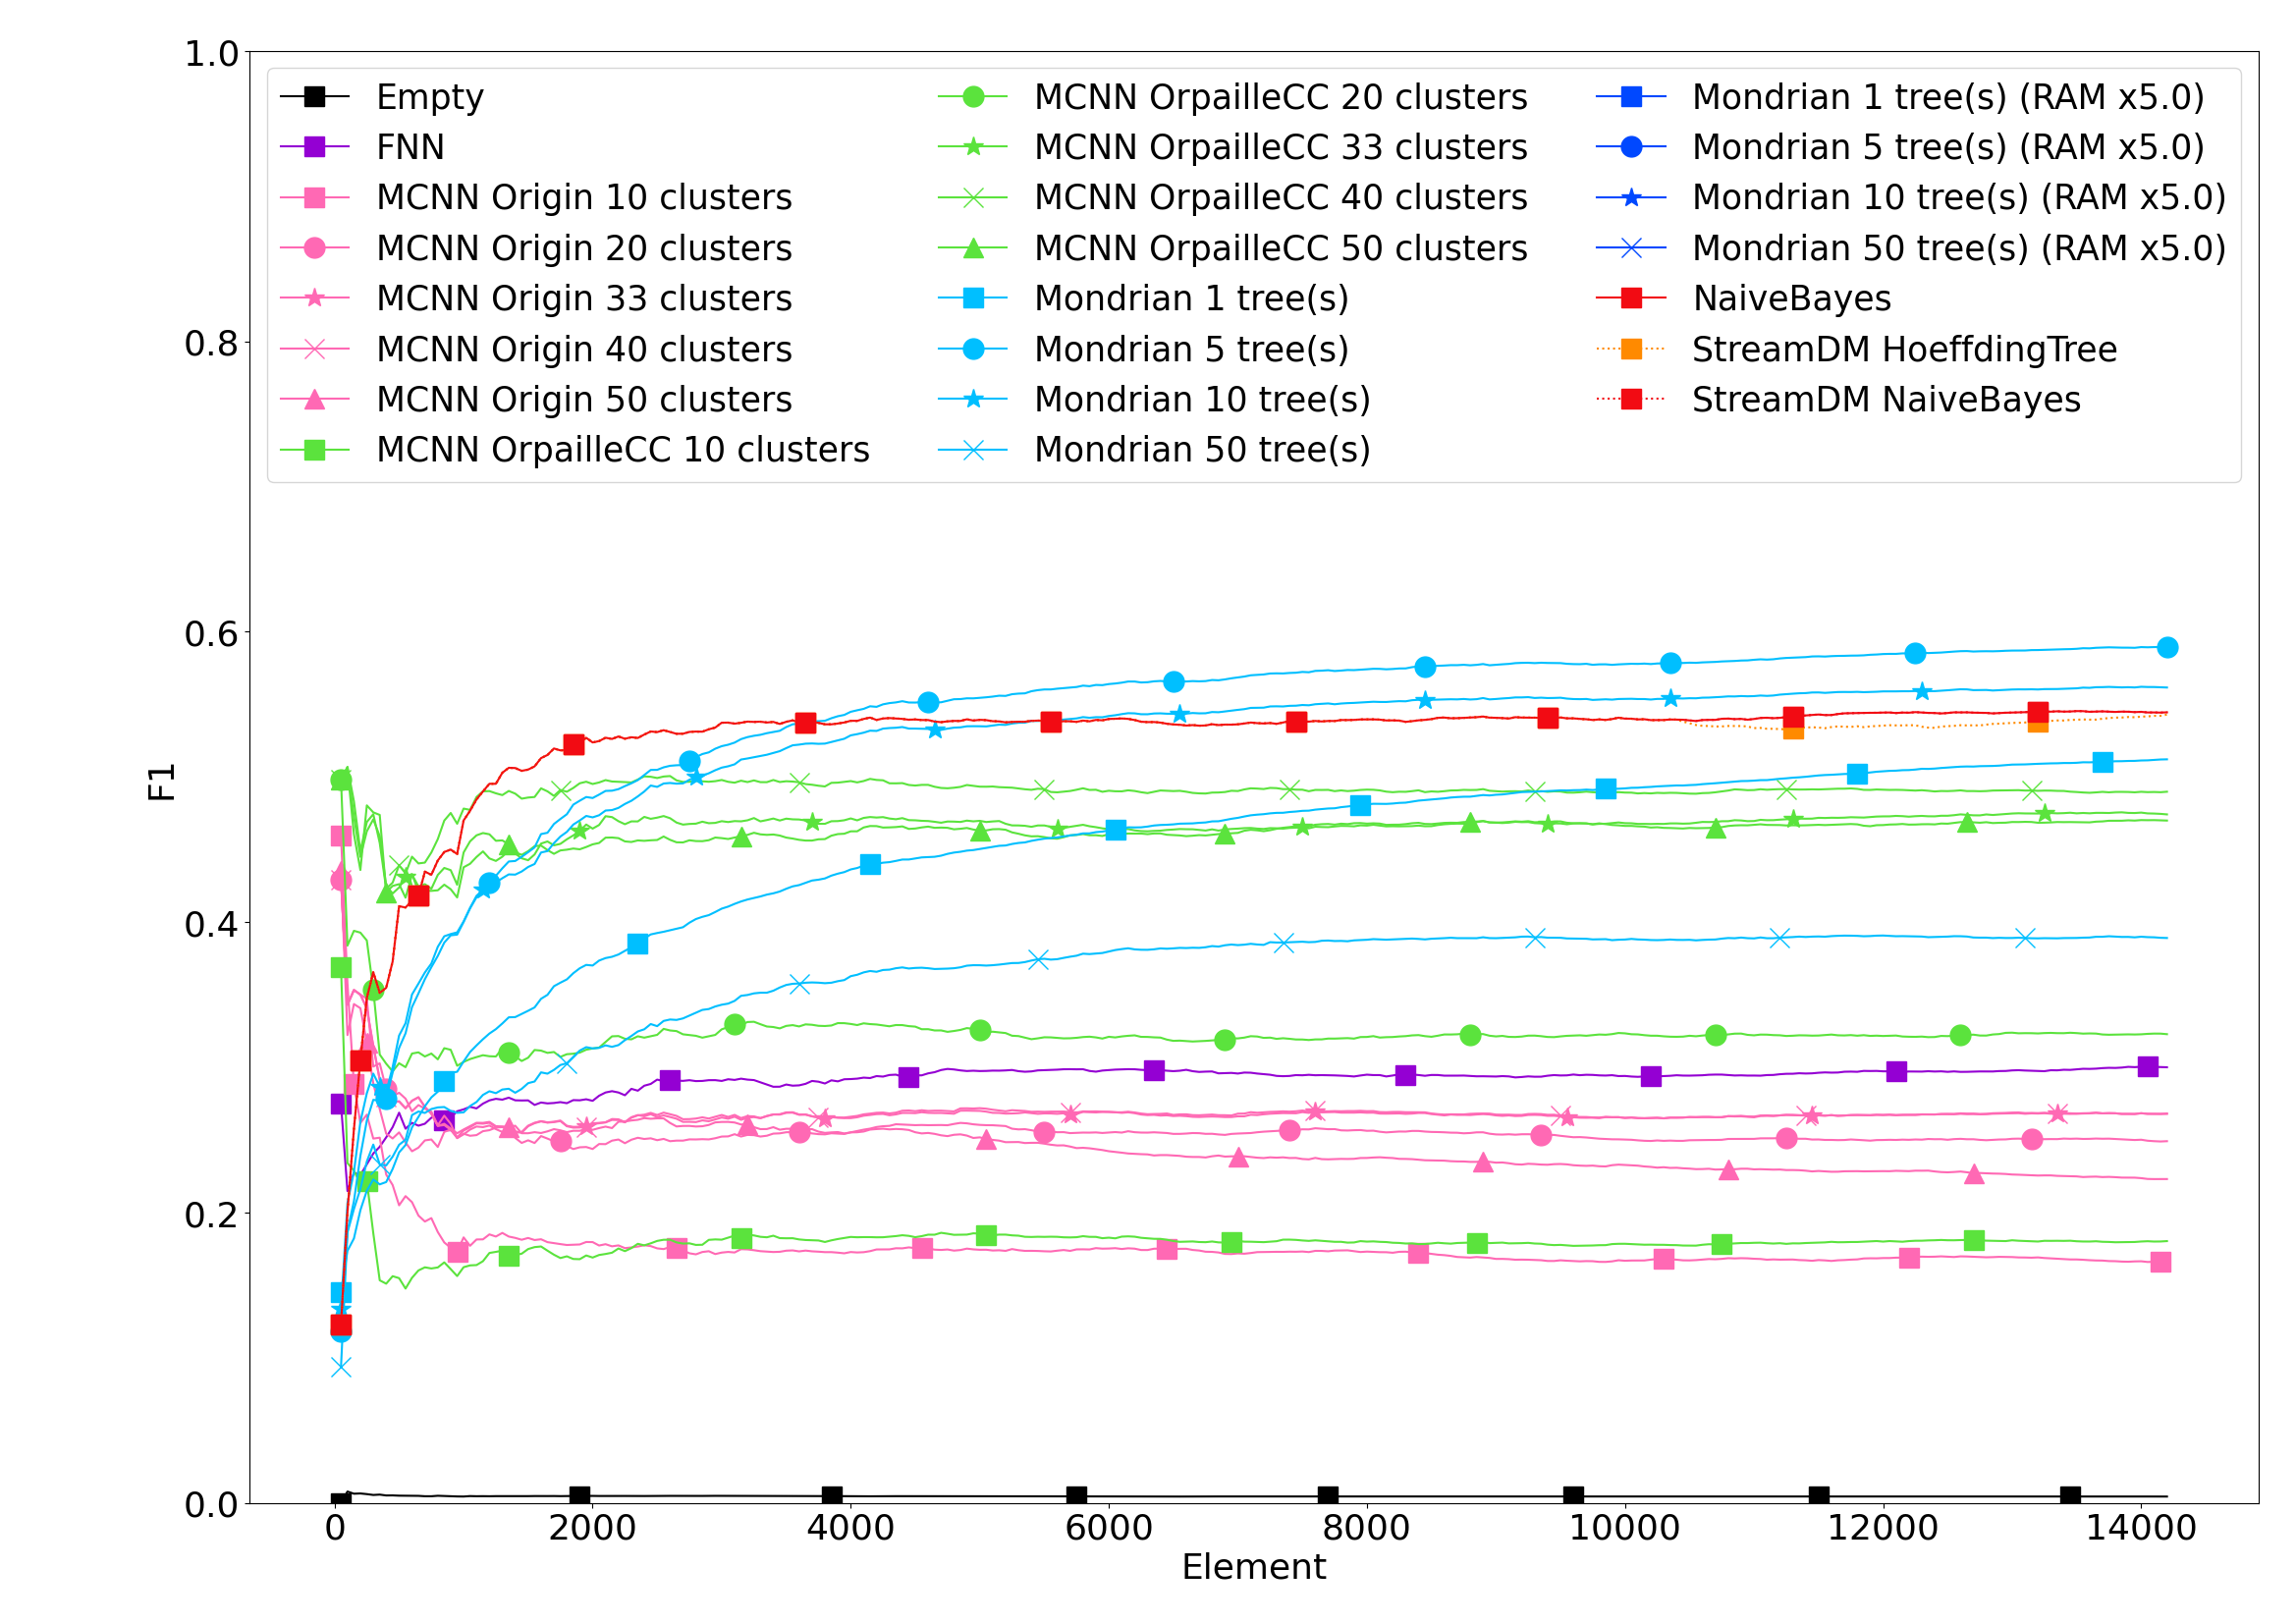
\includegraphics[width=\linewidth]{figures/results/banos_3_f1.png}
		\caption{\banosdataset}
		\label{fig:f1-banos}
	\end{subfigure}
	\begin{subfigure}[t]{.5\linewidth}
		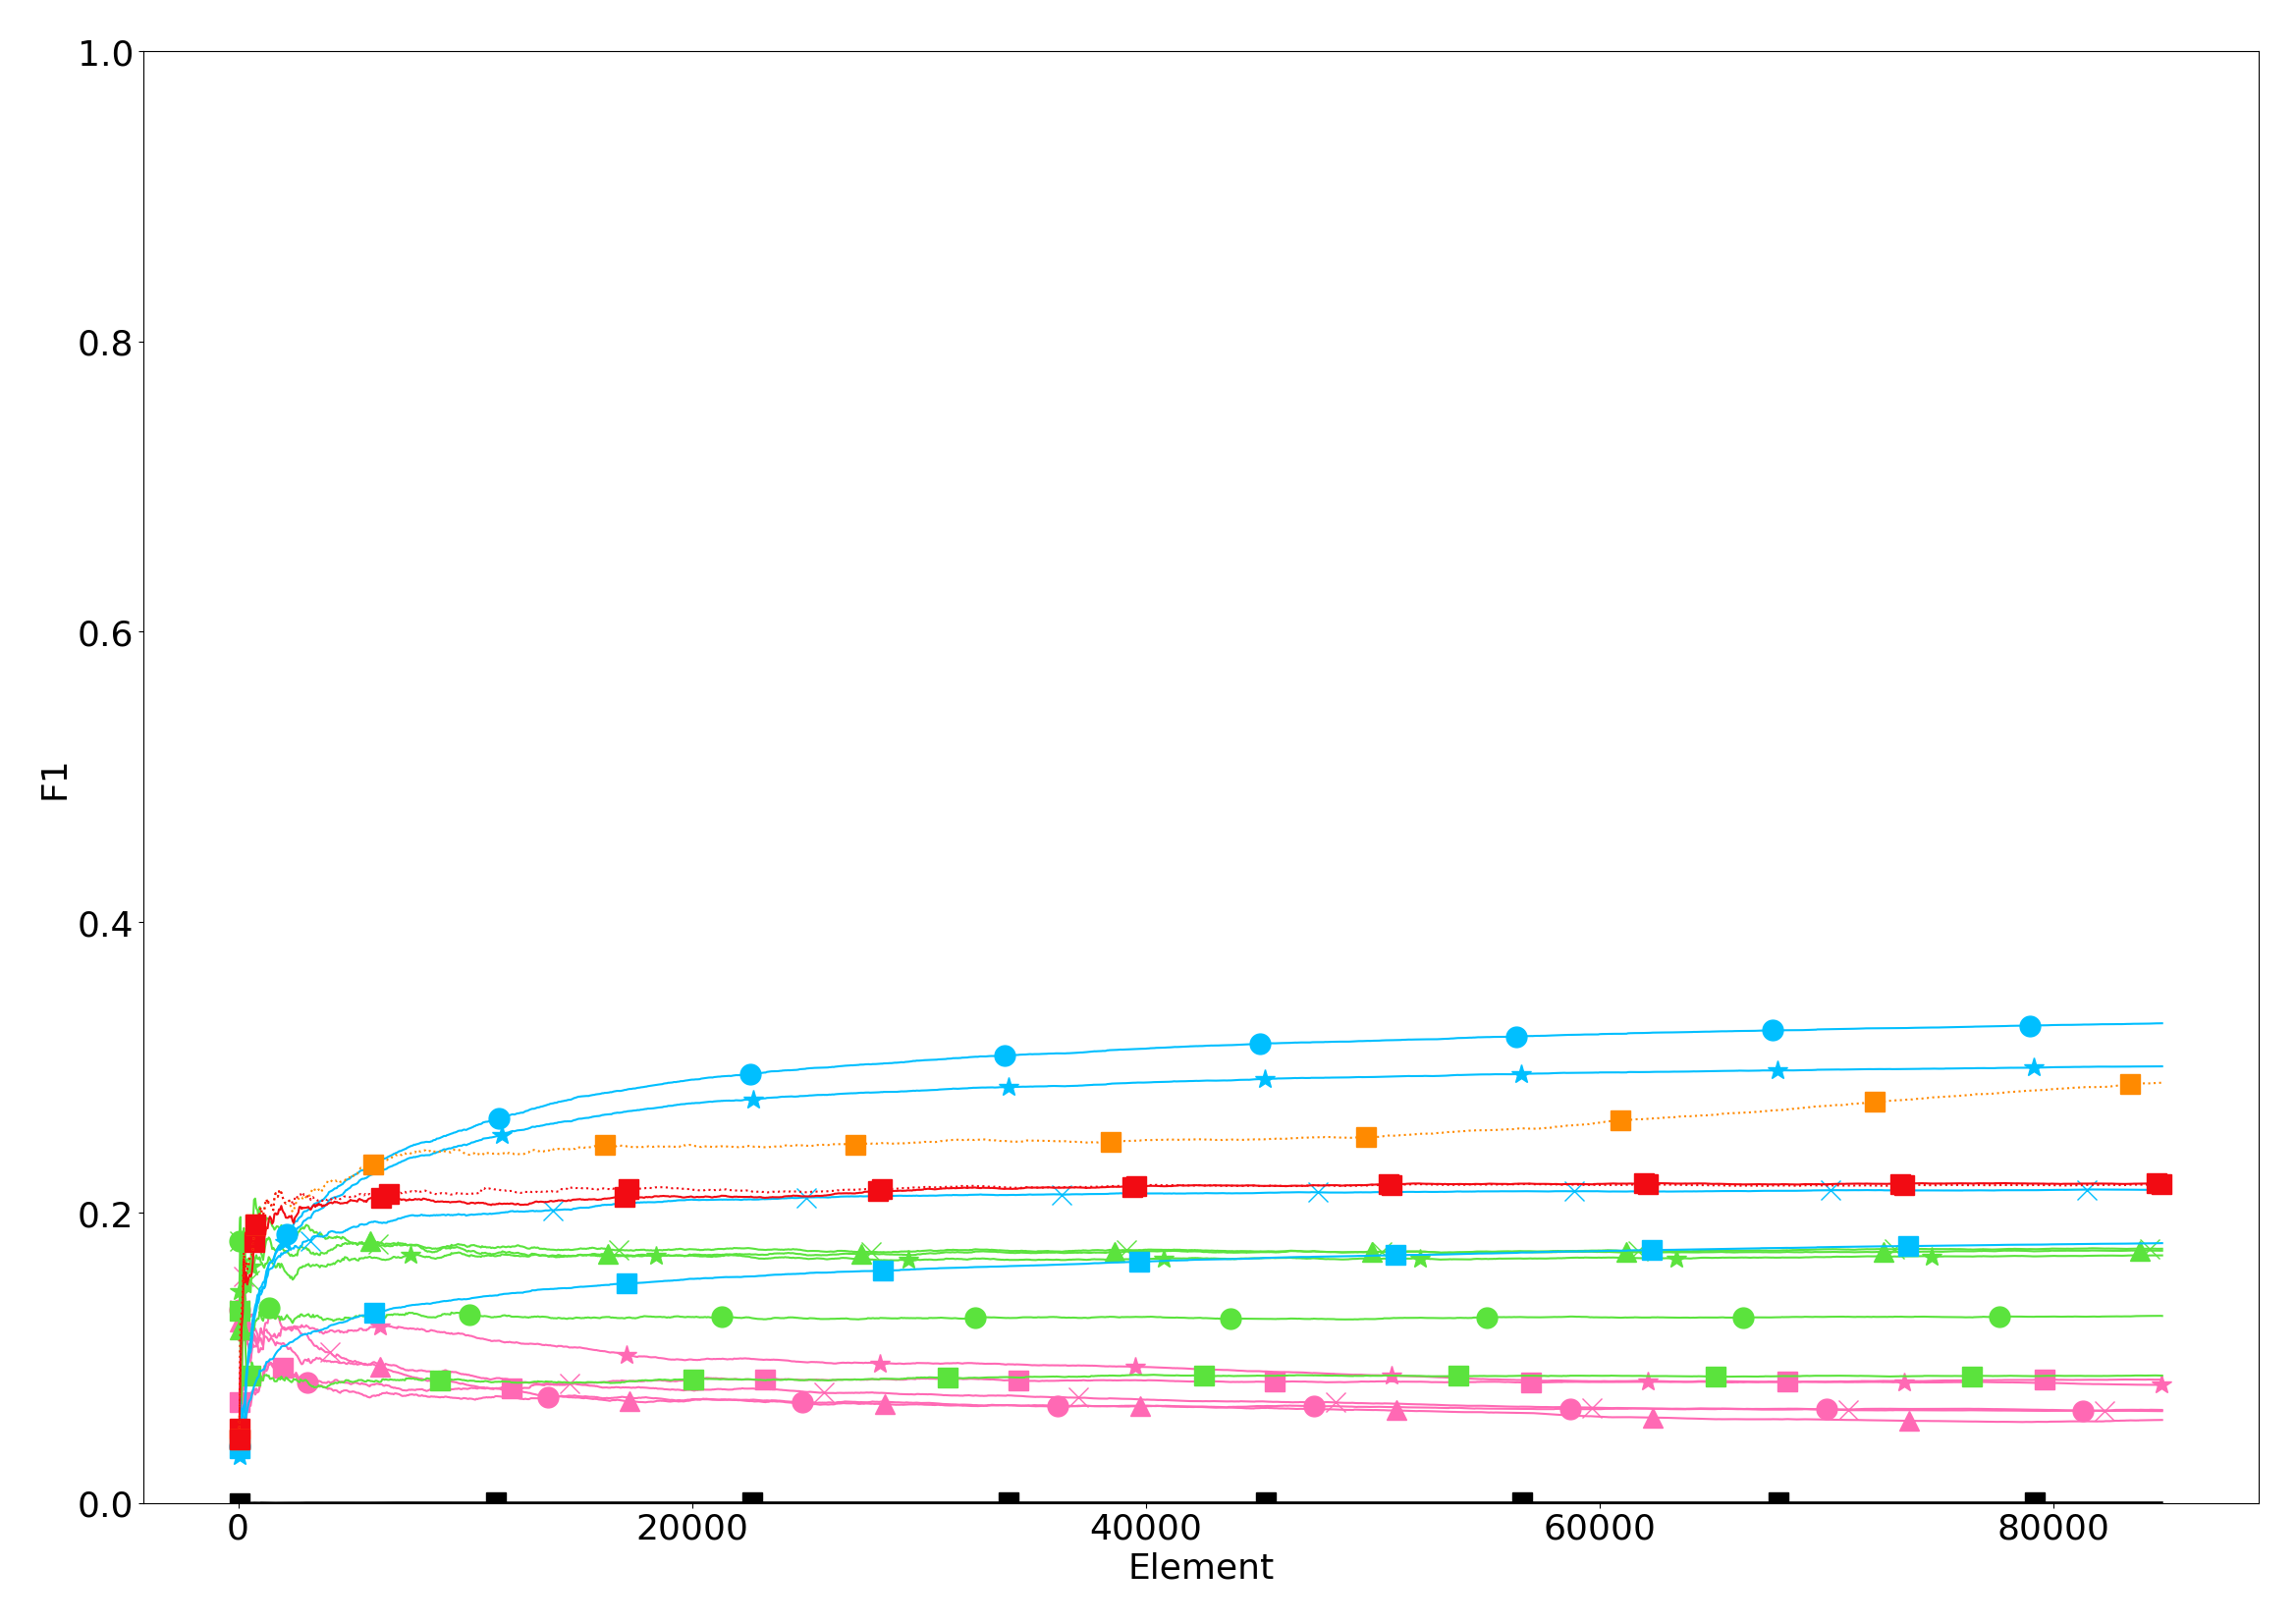
\includegraphics[width=\linewidth]{figures/results/recofit_3_f1.png}
		\caption{\recofitdataset}
		\label{fig:f1-recofit}
	\end{subfigure}
	\begin{subfigure}[t]{.5\linewidth}
		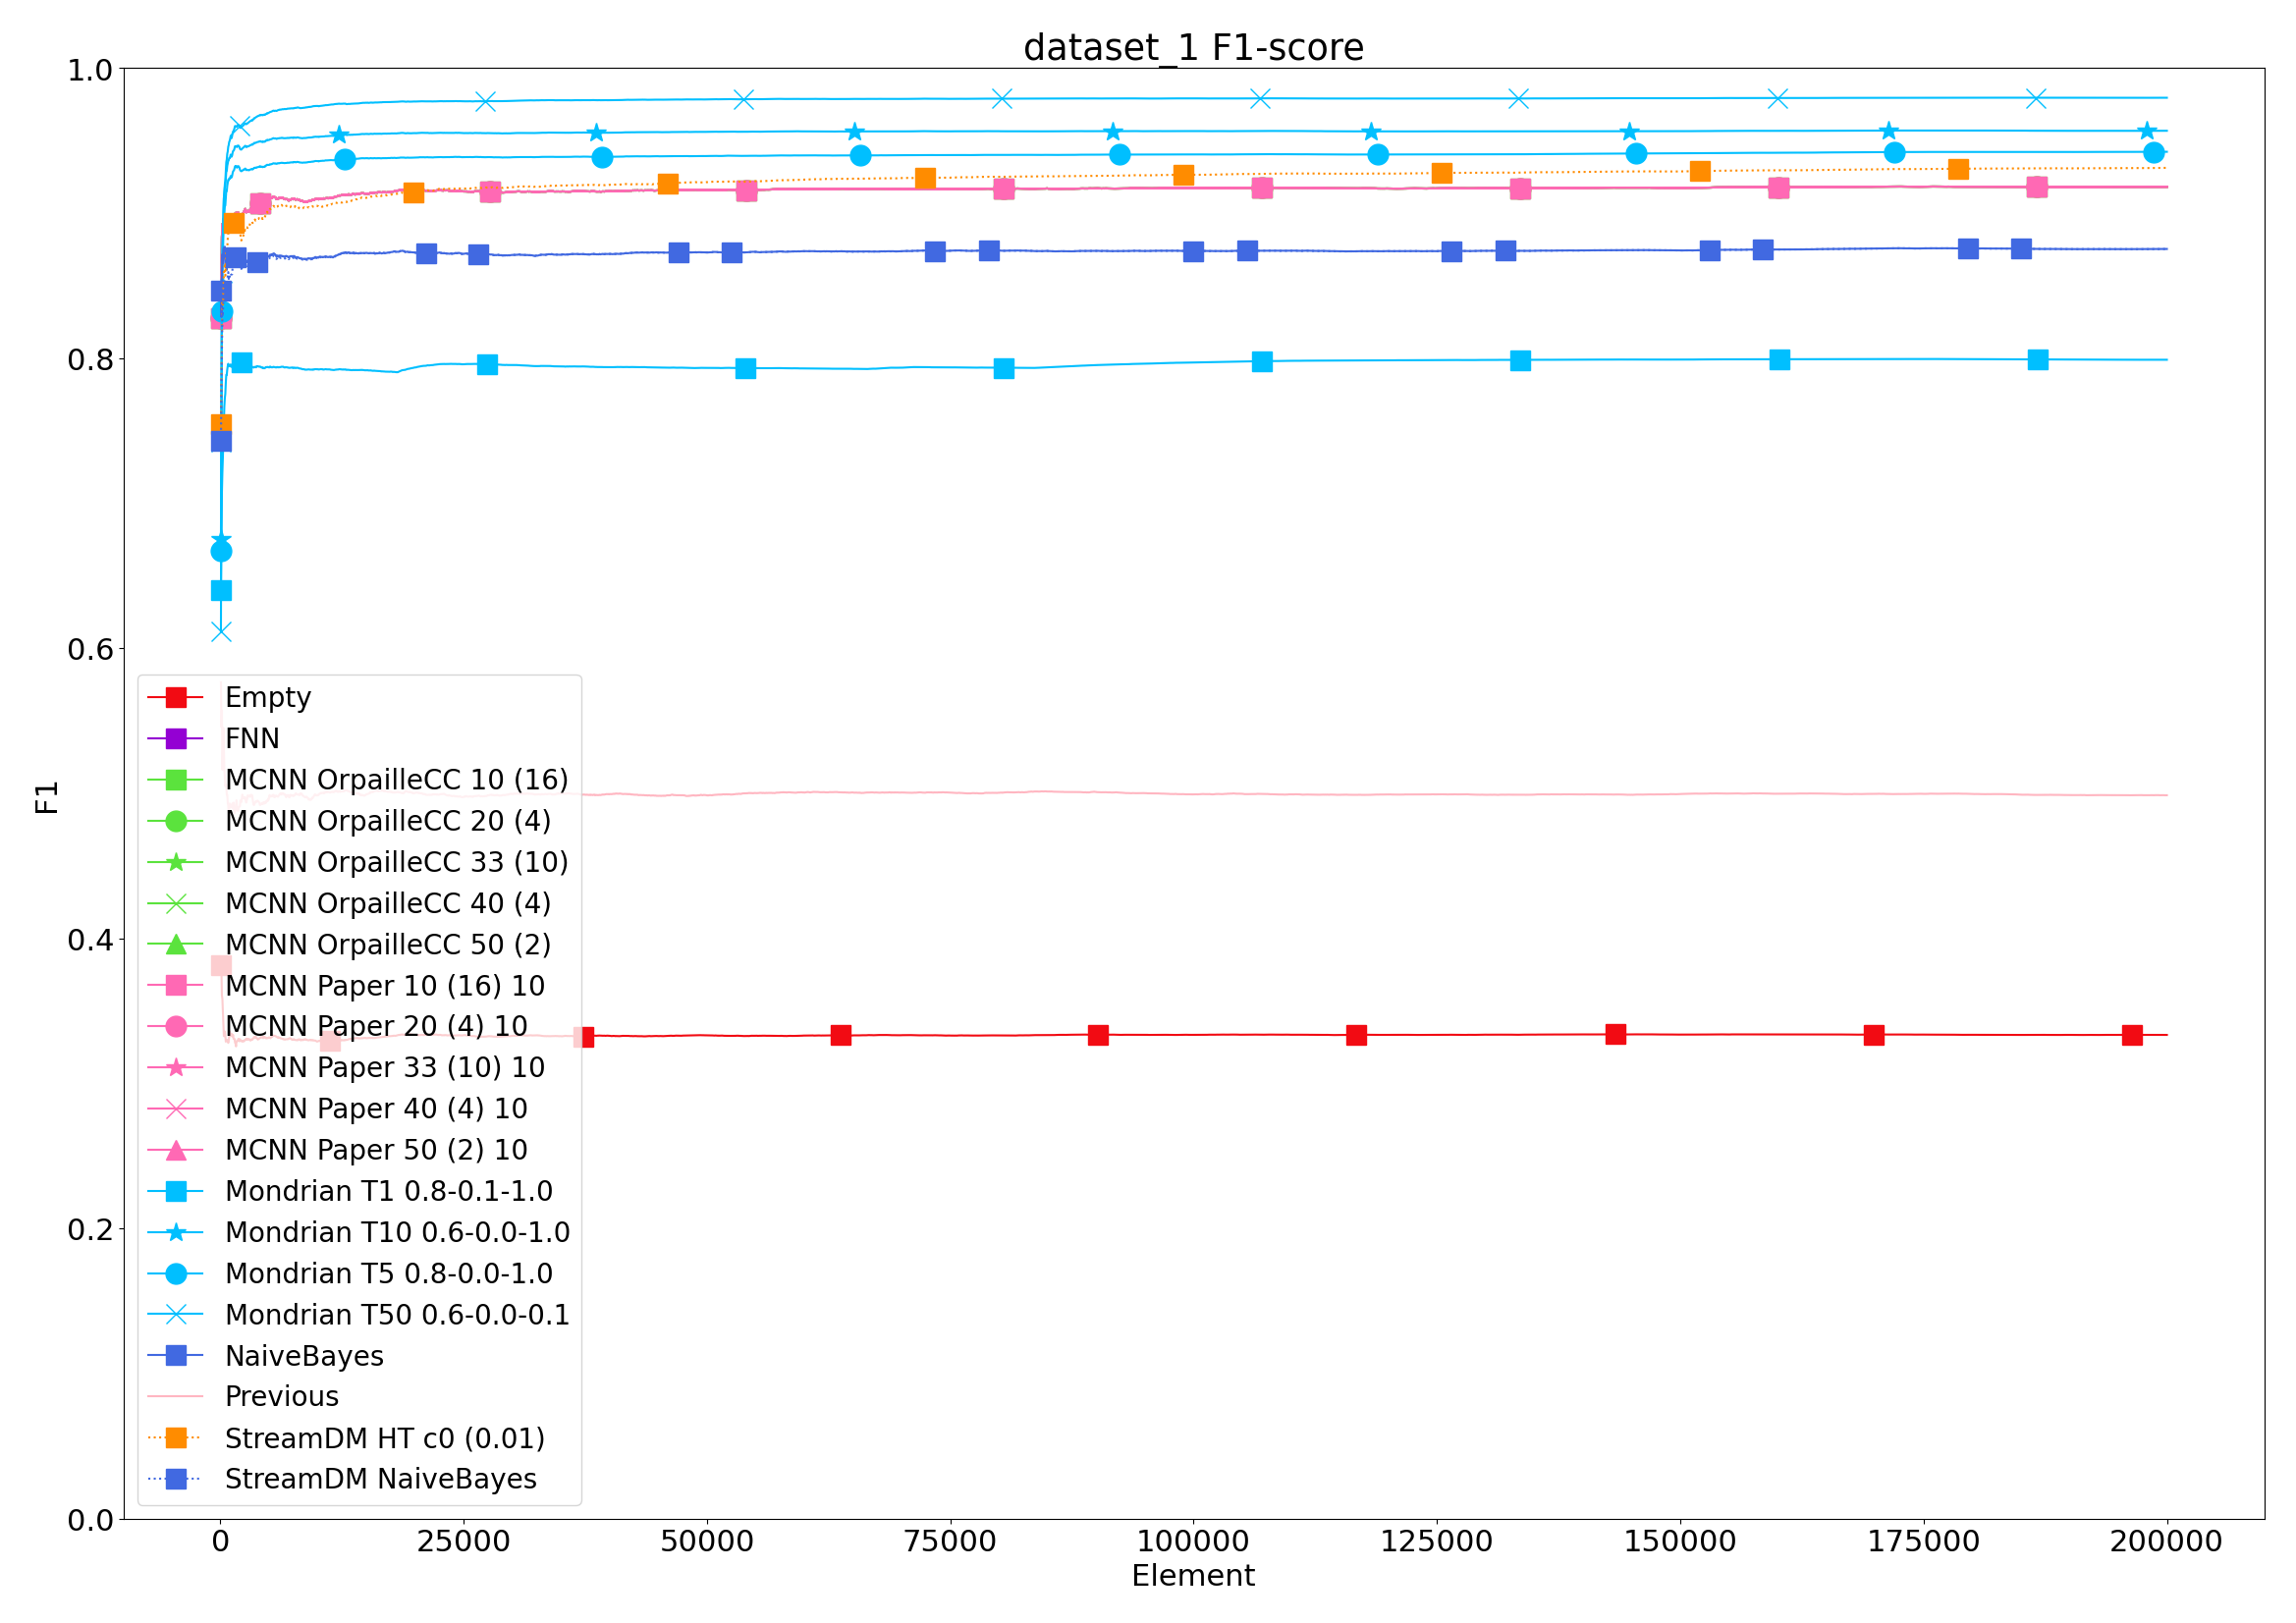
\includegraphics[width=\linewidth]{figures/results/dataset_1_f1.png}
		\caption{Hyperplane}
		\label{fig:f1-dataset_1}
	\end{subfigure}
	\begin{subfigure}[t]{.5\linewidth}
		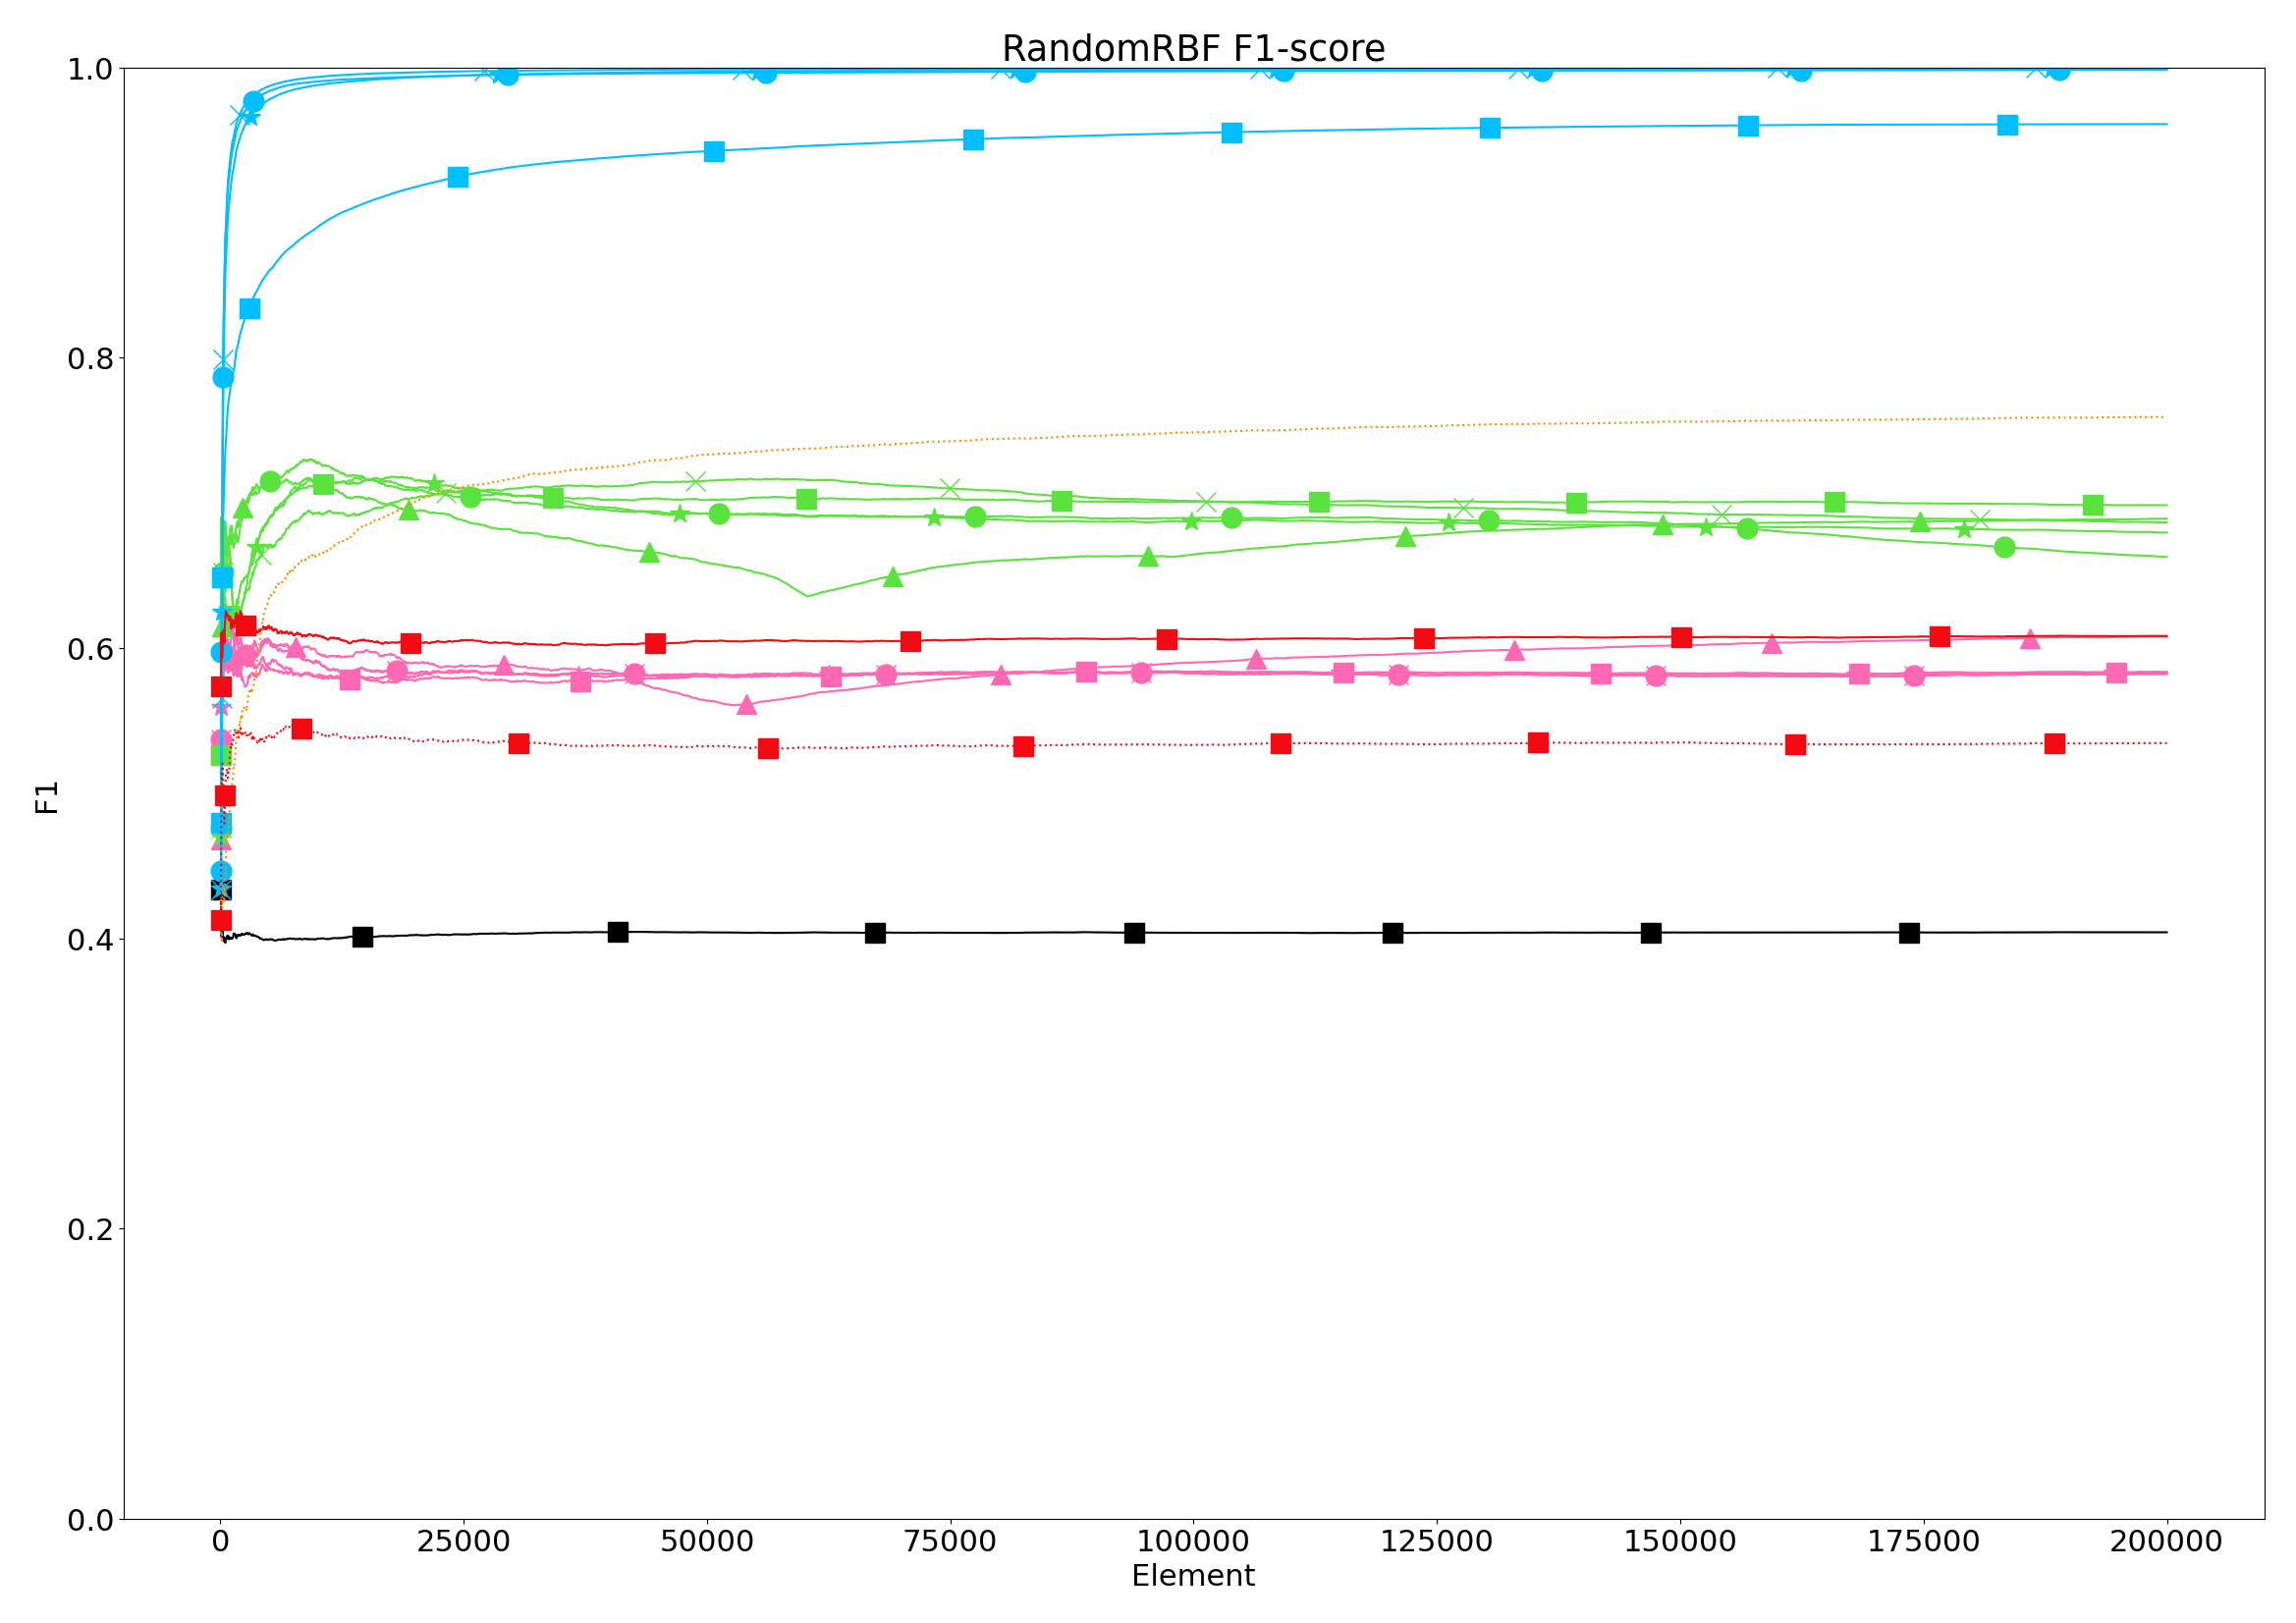
\includegraphics[width=\linewidth]{figures/results/dataset_2_f1.png}
		\caption{RandomRBF}
		\label{fig:f1-dataset_2}
	\end{subfigure}
	\begin{subfigure}[t]{.5\linewidth}
		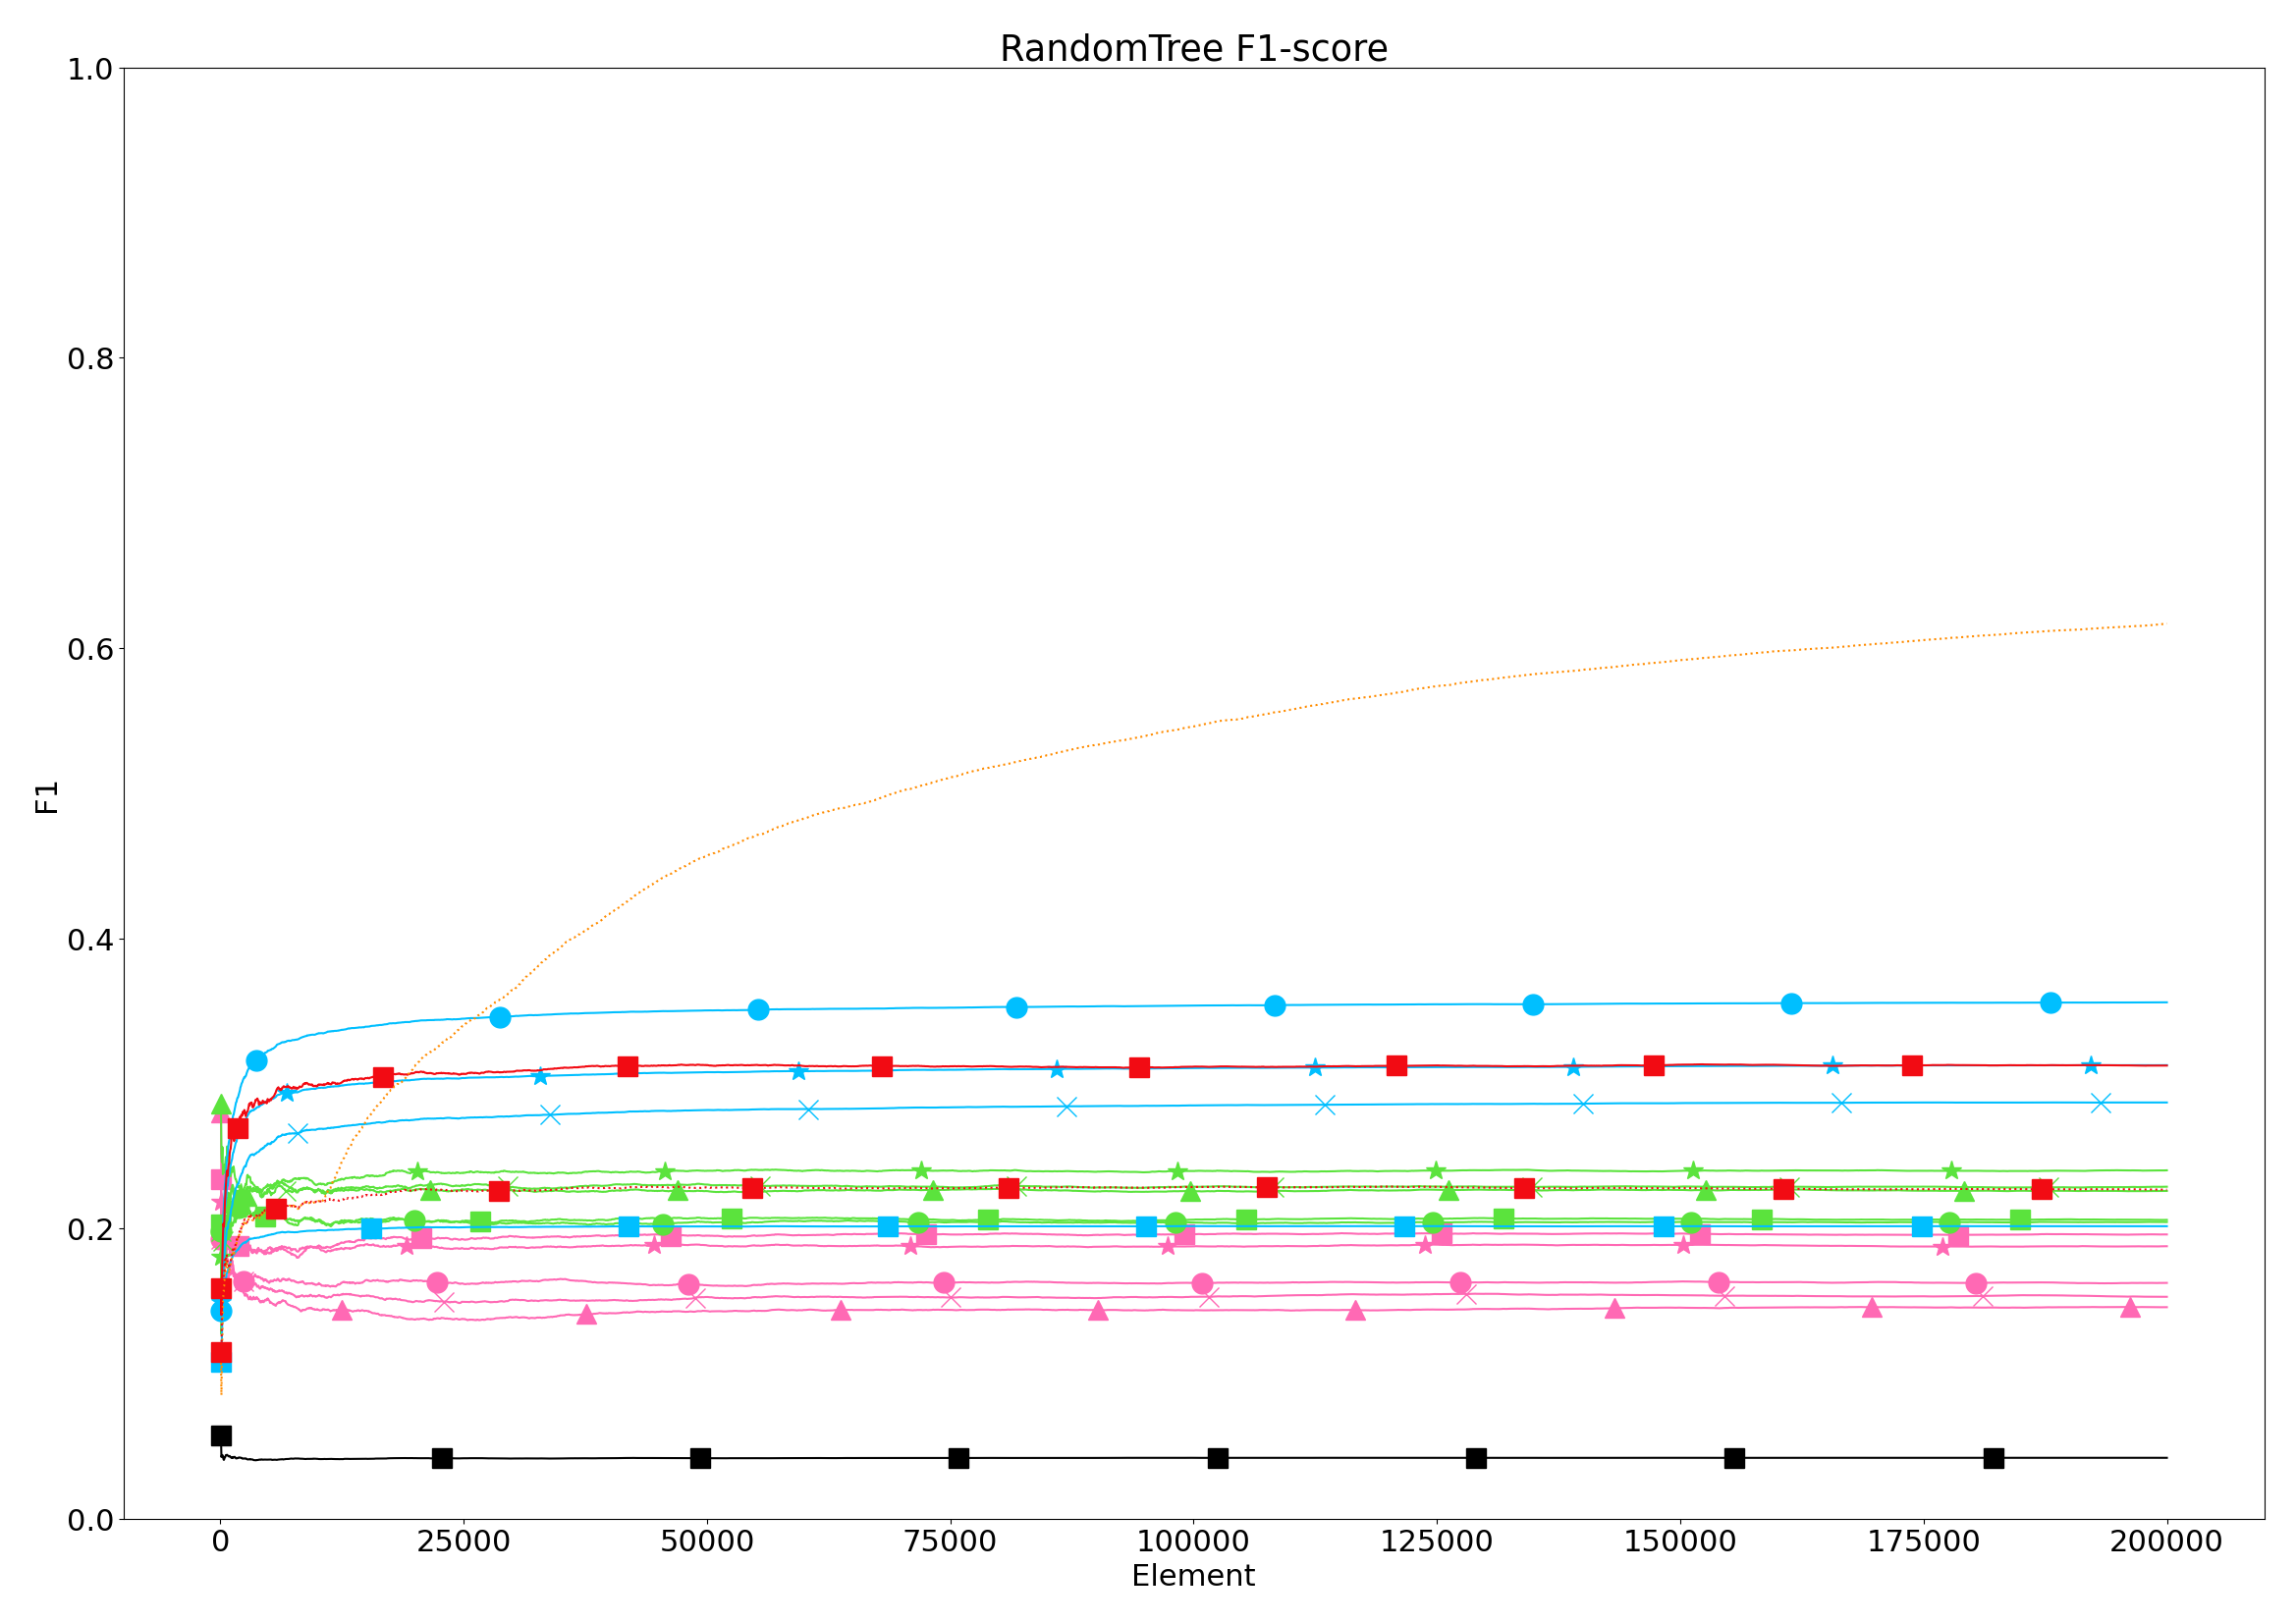
\includegraphics[width=\linewidth]{figures/results/dataset_3_f1.png}
		\caption{RandomTree}
		\label{fig:f1-dataset_3}
	\end{subfigure}
	\begin{subfigure}[t]{.5\linewidth}
		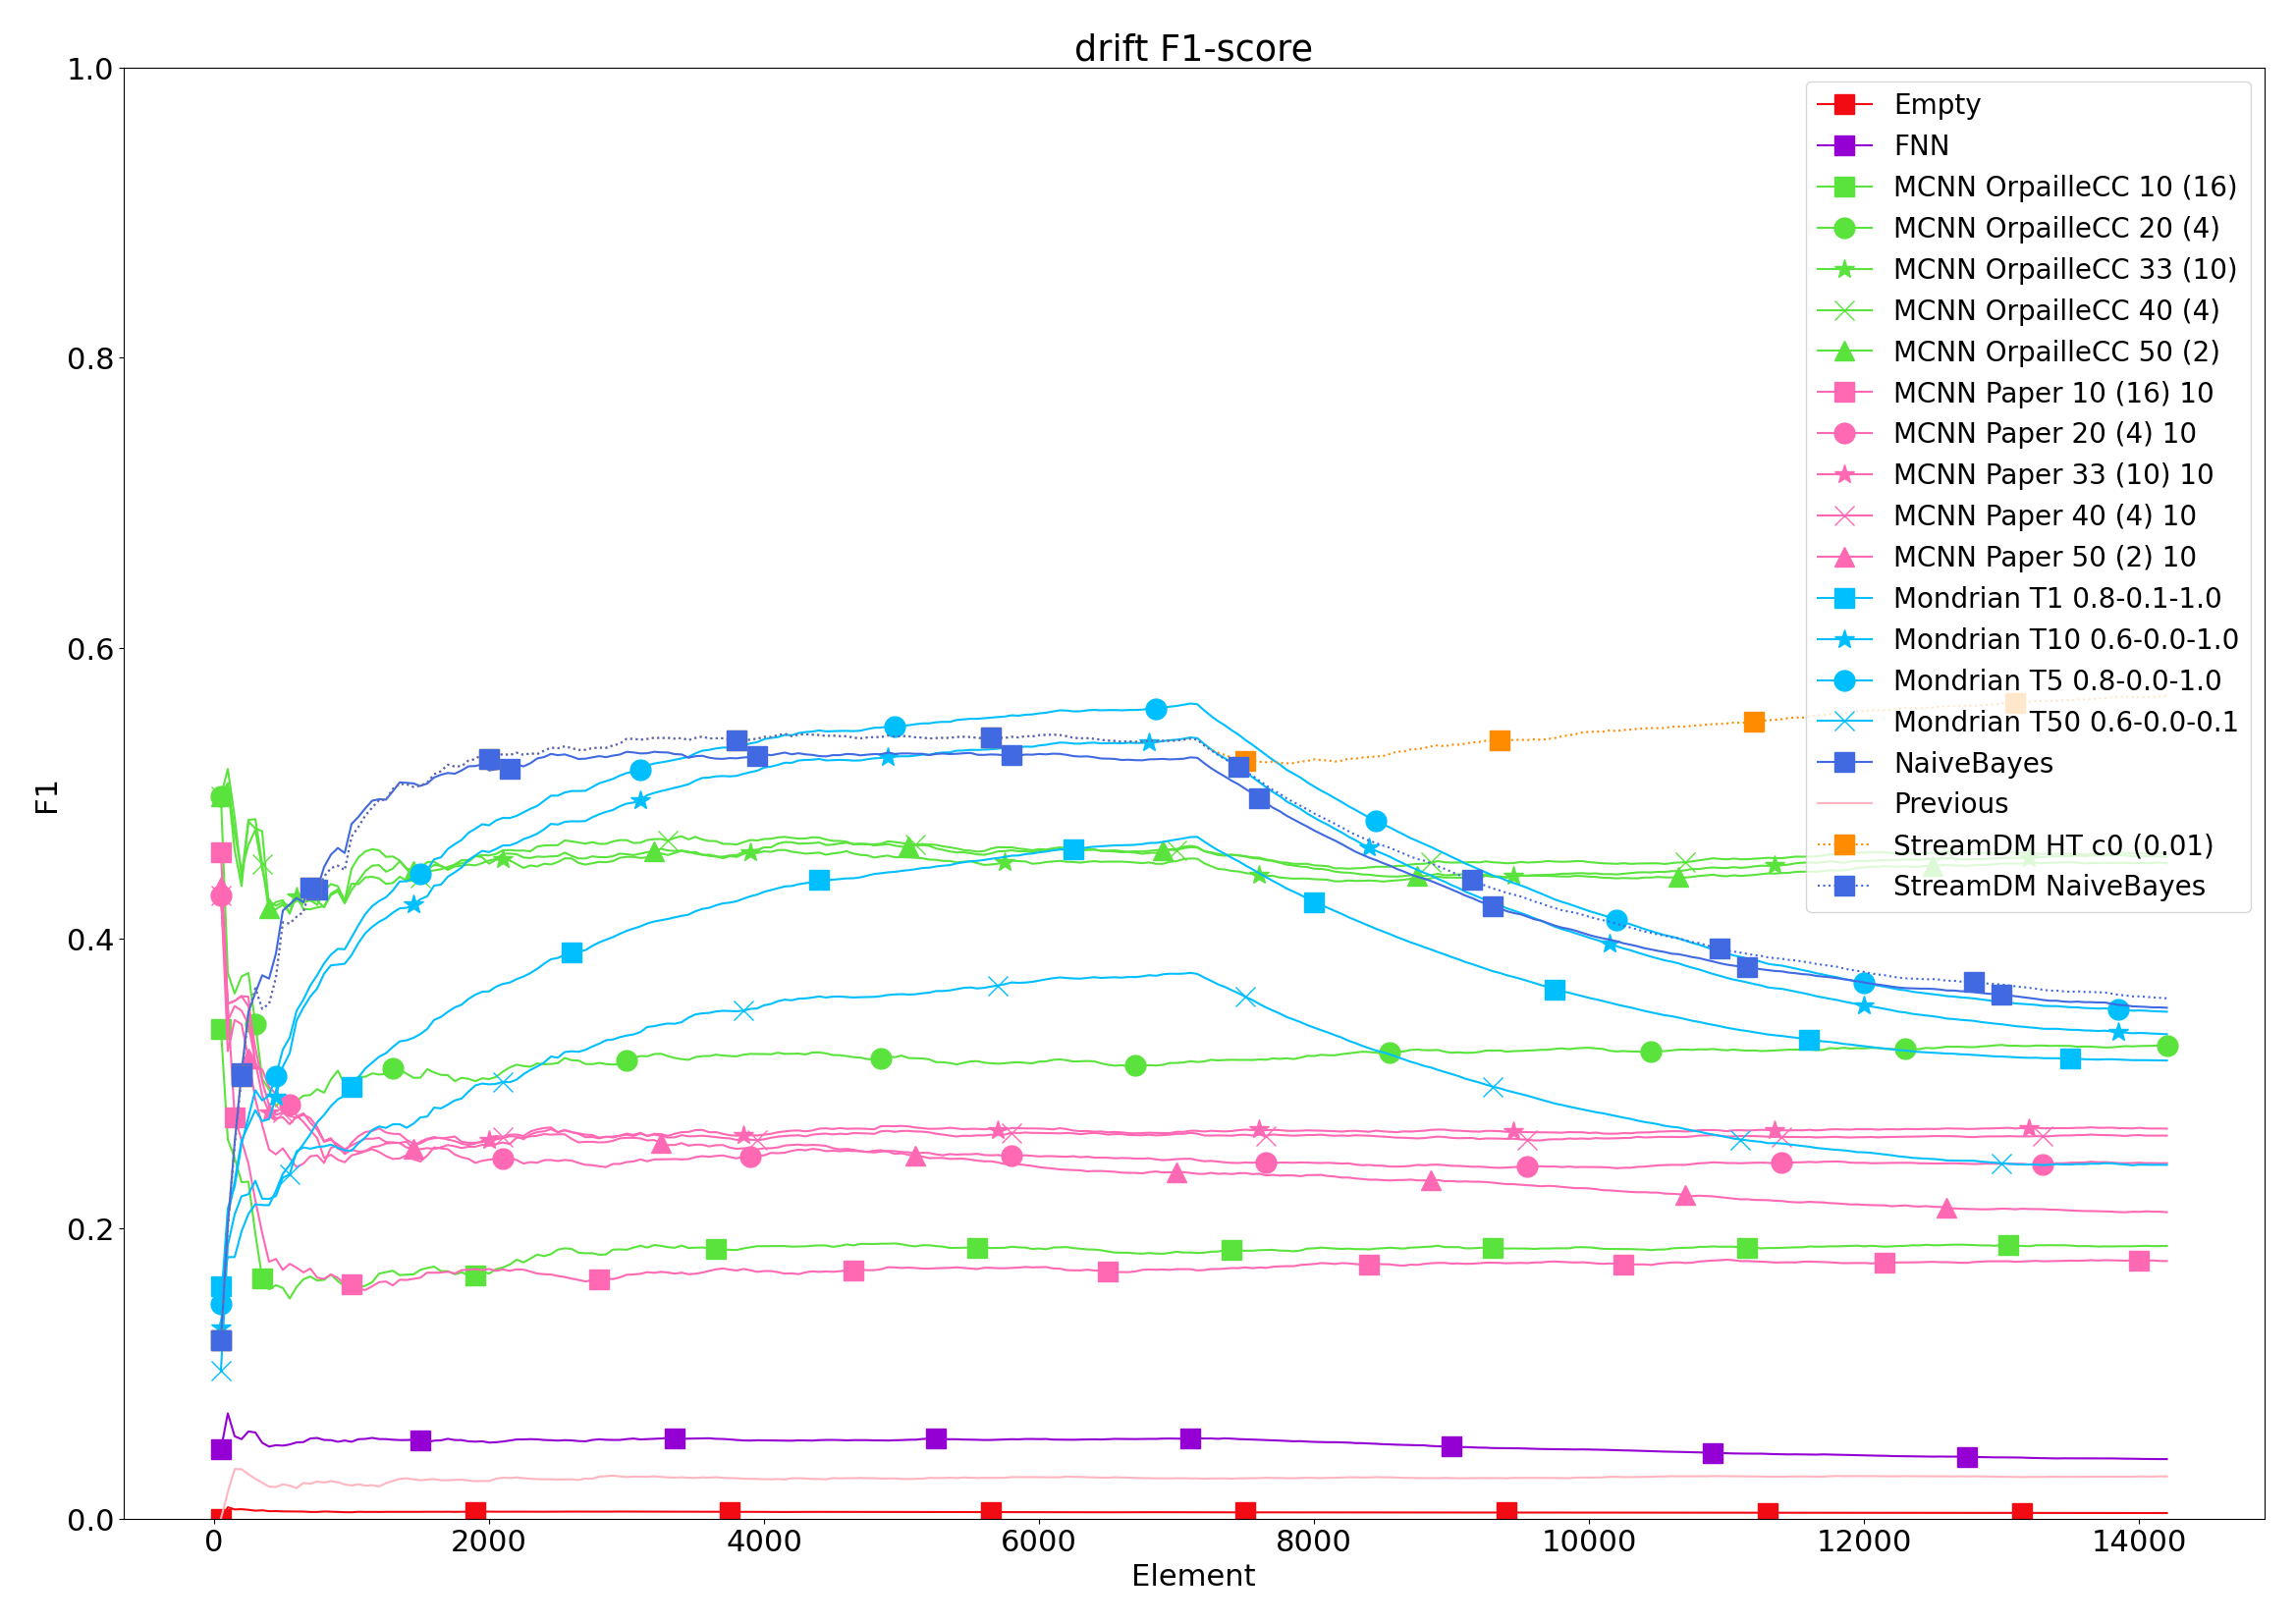
\includegraphics[width=\linewidth]{figures/results/drift_f1.png}
		\caption{Drift}
		\label{fig:f1-drift}
	\end{subfigure}

	\caption{F1-scores on each dataset.}
	\label{fig:f1}
\end{figure*}

Regarding the actual F1-scores values, we notice wide disparities between the
datasets. On the two synthetic datasets Hyperplane and RandomRBF, Mondrian
reaches an F1-score higher than 0.95. On the other hand, with the
\banosdataset, the f1-score decreases between 0.5 and 0.6.  Finally, it barely
reaches 0.3 on \recofitdataset and RandomTree.

A similar observation can be made about naïve Bayes classifiers. Higher
F1-scores with the Hyperplane, medium performance with \banosdataset and
RandomRBF, and poor results with \recofitdataset and RandomTree.

Concerning the StreamDM HoeffdingTree algorithm, we can see that it matches
very closely the StreamDM naïve Bayes. It happens because the HoeffdingTree
uses a naïve Bayes in the leaves. However, we notice that the two start
diverging because the HoeffdingTree improves by reshaping its tree structure.
This is caused by either a suffisant amount of element or by a drift.

In Figure~\ref{fig:f1-banos}, there are two types of MCNN: MCNN-Origin and
MCNN-OrpailleCC.  Both algorithm are implemented in the library OrpailleCC,
however, MCNN-Origin strictly follows the algorithm described in~\cite{mc-nn}
whereas MCNN-OrpailleCC tweaks this algorithm to ensure a fixed memory
footprint. The difference appears on how micro-clusters are removed.
MCNN-Origin removes a micro-cluster when its participation falls below a
threshold given by the user while MCNN-OrpailleCC removes the micro-cluster with
the least participation when the maximum number of micro-cluster is reached and
a new micro-cluster has to be introduced.

Figures~\ref{fig:f1} shows that in all cases, MCNN-OrpailleCC achieves
better performance than its MCNN-Origin counter-part. Additionally, most of
the time, any MCNN-OrpailleCC performs better than all MCNN-Origin.

We note that on the real datasets (\banosdataset and \recofitdataset), the
naïve Bayes algorithm learns faster than the Mondrian. The Mondrian catches up
after a few thousand elements. Even though it is difficult to notice on most of
the datasets, we can see on \banosdataset that MCNN OrpailleCC leans faster
than the naïve Bayes when there are less than a thousand elements.

Surprisingly, we observe that using 50 trees with the Mondrian algorithm shows worse
f1-scores than using 5 or 10. These unexpected results appear because the
Mondrian implementation forces a fixed memory footprint. Therefore, the tree
growth is blocked when there is not enough memory. Because 50 trees fill the
memory faster than 10 or 5 trees, the classifier adaptation is blocked faster,
when the trees have not learned enough from the data. However, when the memory
available is increased, using 50 trees achieve better f1-scores than using 10
trees.

Figure~\ref{fig:f1-drift} shows the F1-score when an artificial drift is
applied to the \banosdataset. We observe that the f1-score of the Mondrian
algorithm as well as the naïve Bayes suffer from the drift and they cannot adapt
to it. We also note that after a small set back, the HoeffdingTree algorithm
gets its f1-score to increase again. Finally, we barely notice any change on
the f1-score of the MCNNs. Only the highest MCNN (MCNN-OrpailleCC with 33, 40,
and 50 clusters) have a slight decrease.
Note that the difficulties of Mondrian to adapt to the drift can be attributed
to two factors. First, because Mondrian cannot change the parts of the tree that
already exist even though it can reshape the tree. Second, because when the
memory limit is reached, it is not able to grow anymore, thus it cannot reshape
the tree structure.

Finally, we notice that the two naïve Bayes remain close on the two real
datasets: \banosdataset and \recofitdataset. This suggests that the two
implementations are similar, but SreamDM implements additional mechanisms.


\subsection{Power}
\label{sec:result-power}
Figure~\ref{fig:power} shows the power usage of each classifier on four
datasets. We notice that the classifier has little impact on the
power usage which remains close to 102 watts.

\begin{figure*}
	\begin{subfigure}[t]{.5\linewidth}
		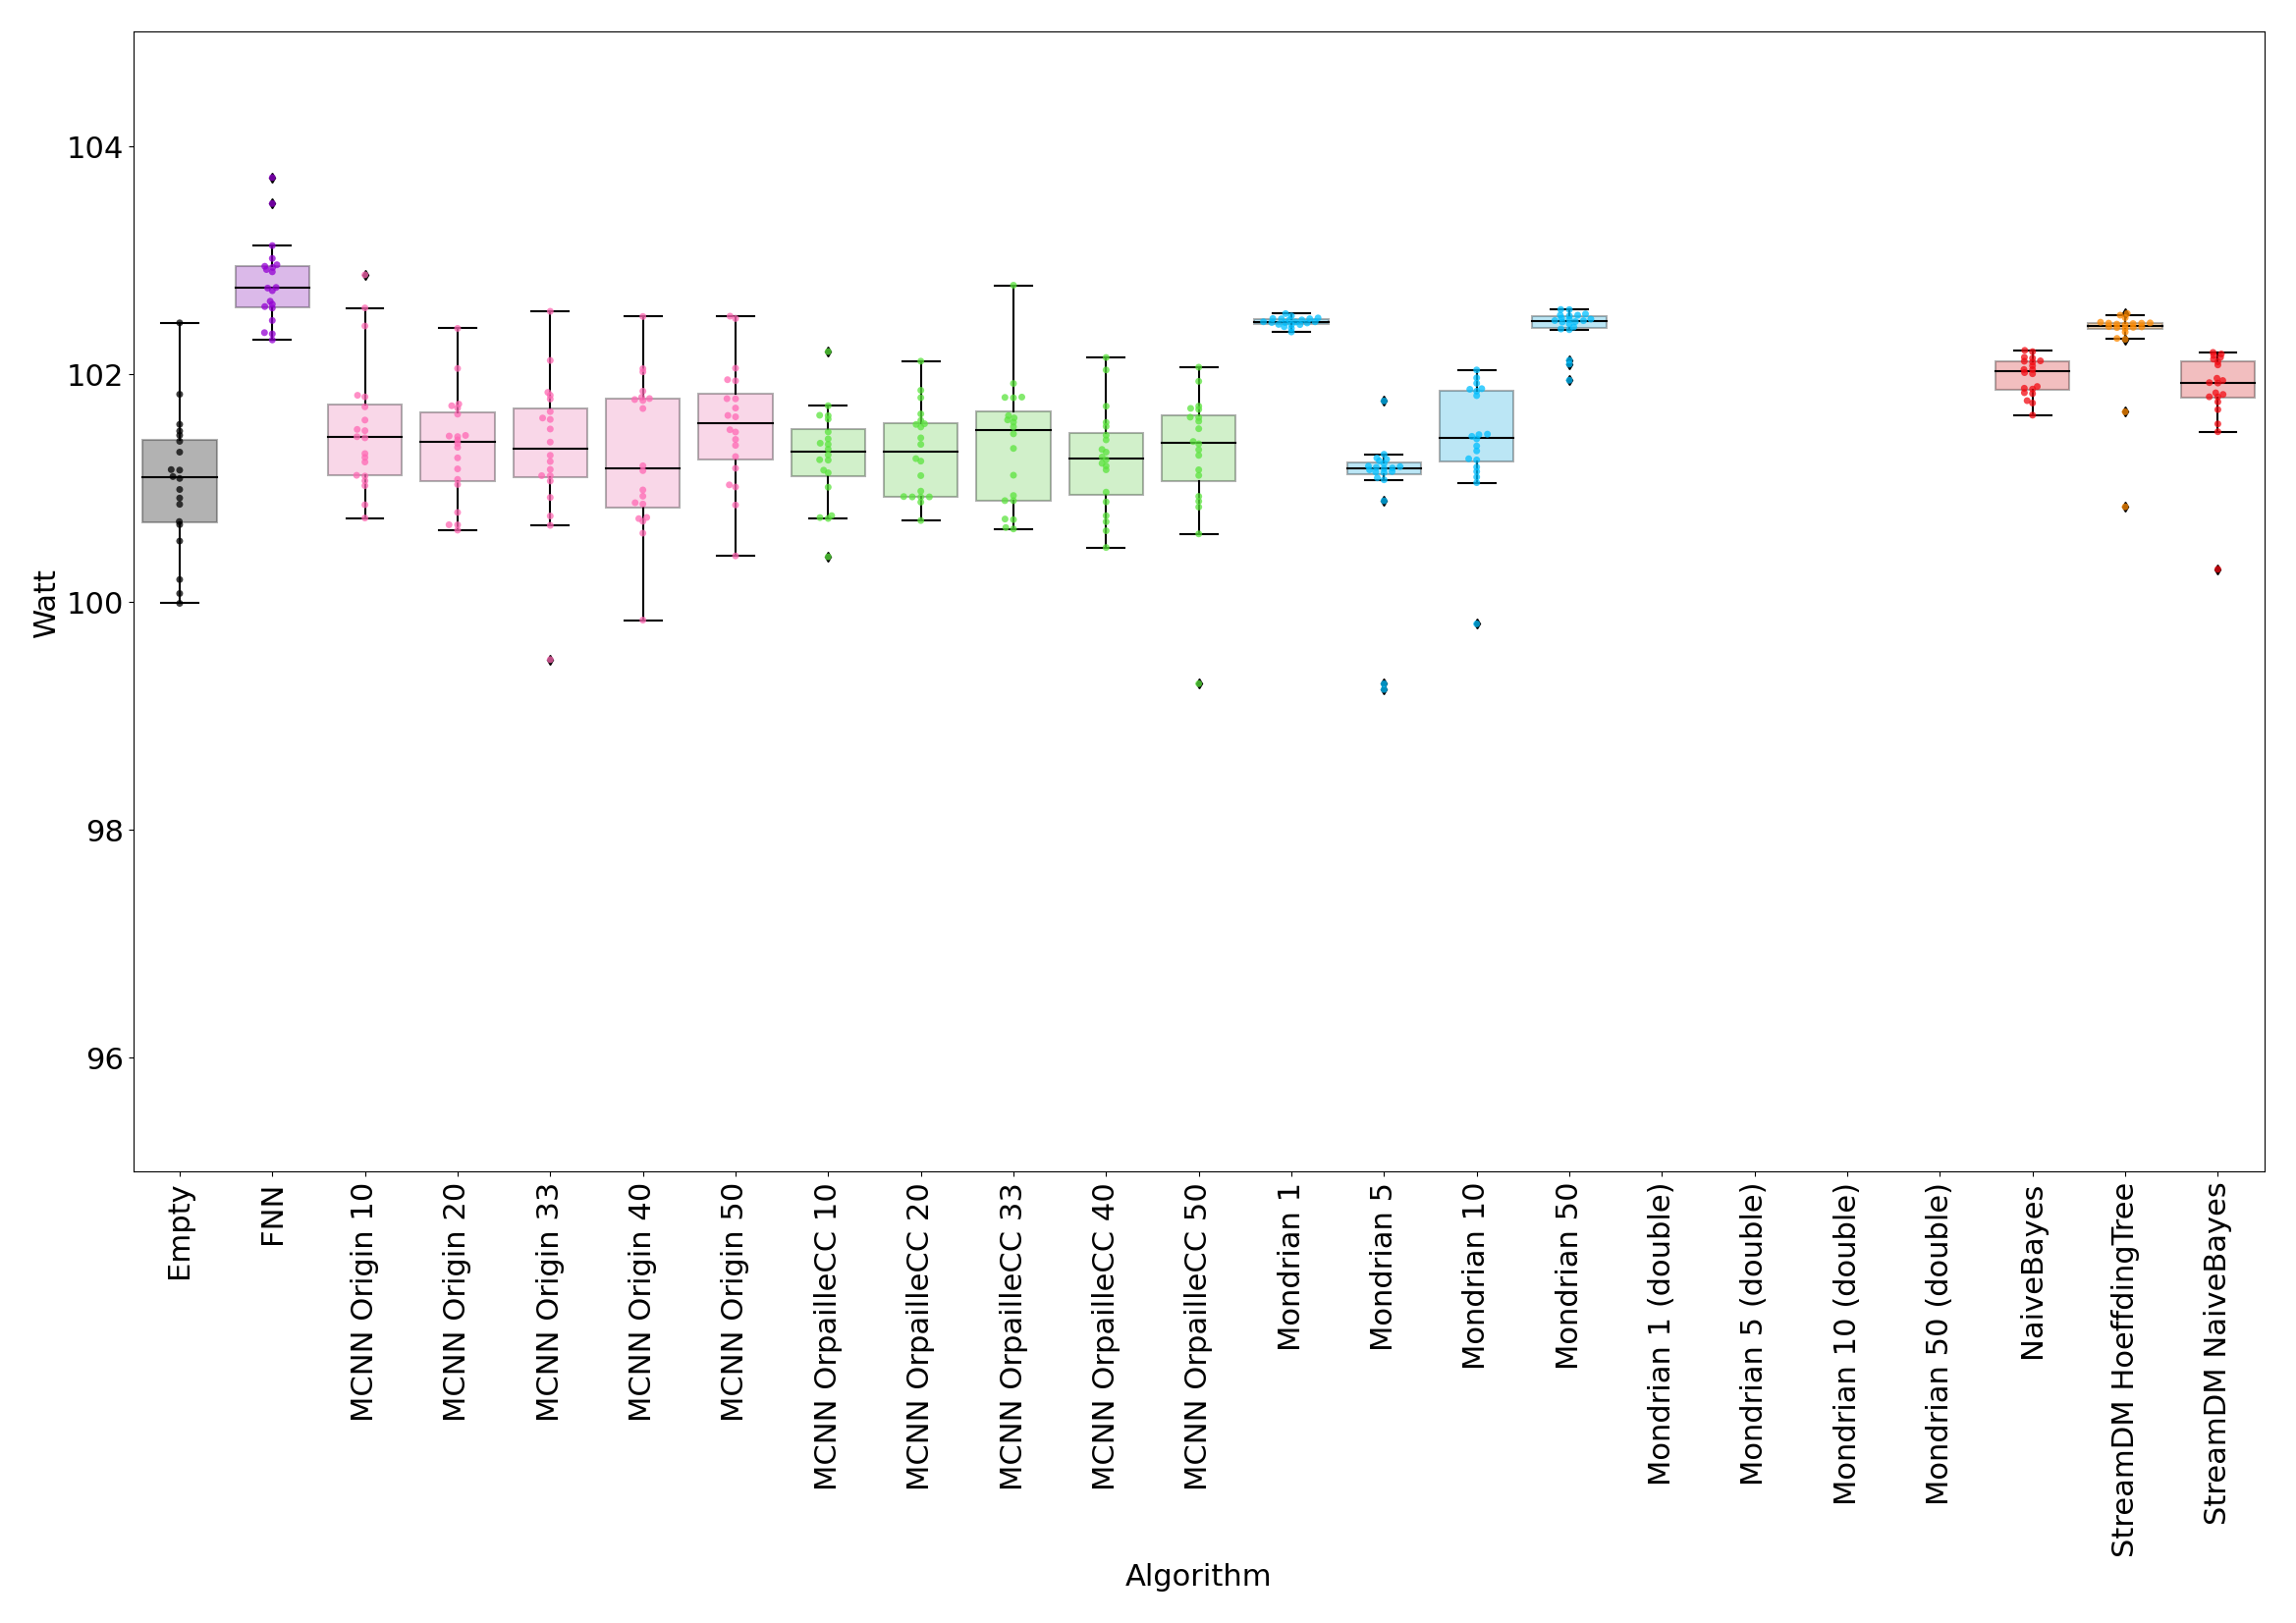
\includegraphics[width=\linewidth]{figures/results/banos_3_watt.png}
		\caption{\banosdataset}
		\label{fig:power-banos}
	\end{subfigure}
	\begin{subfigure}[t]{.5\linewidth}
		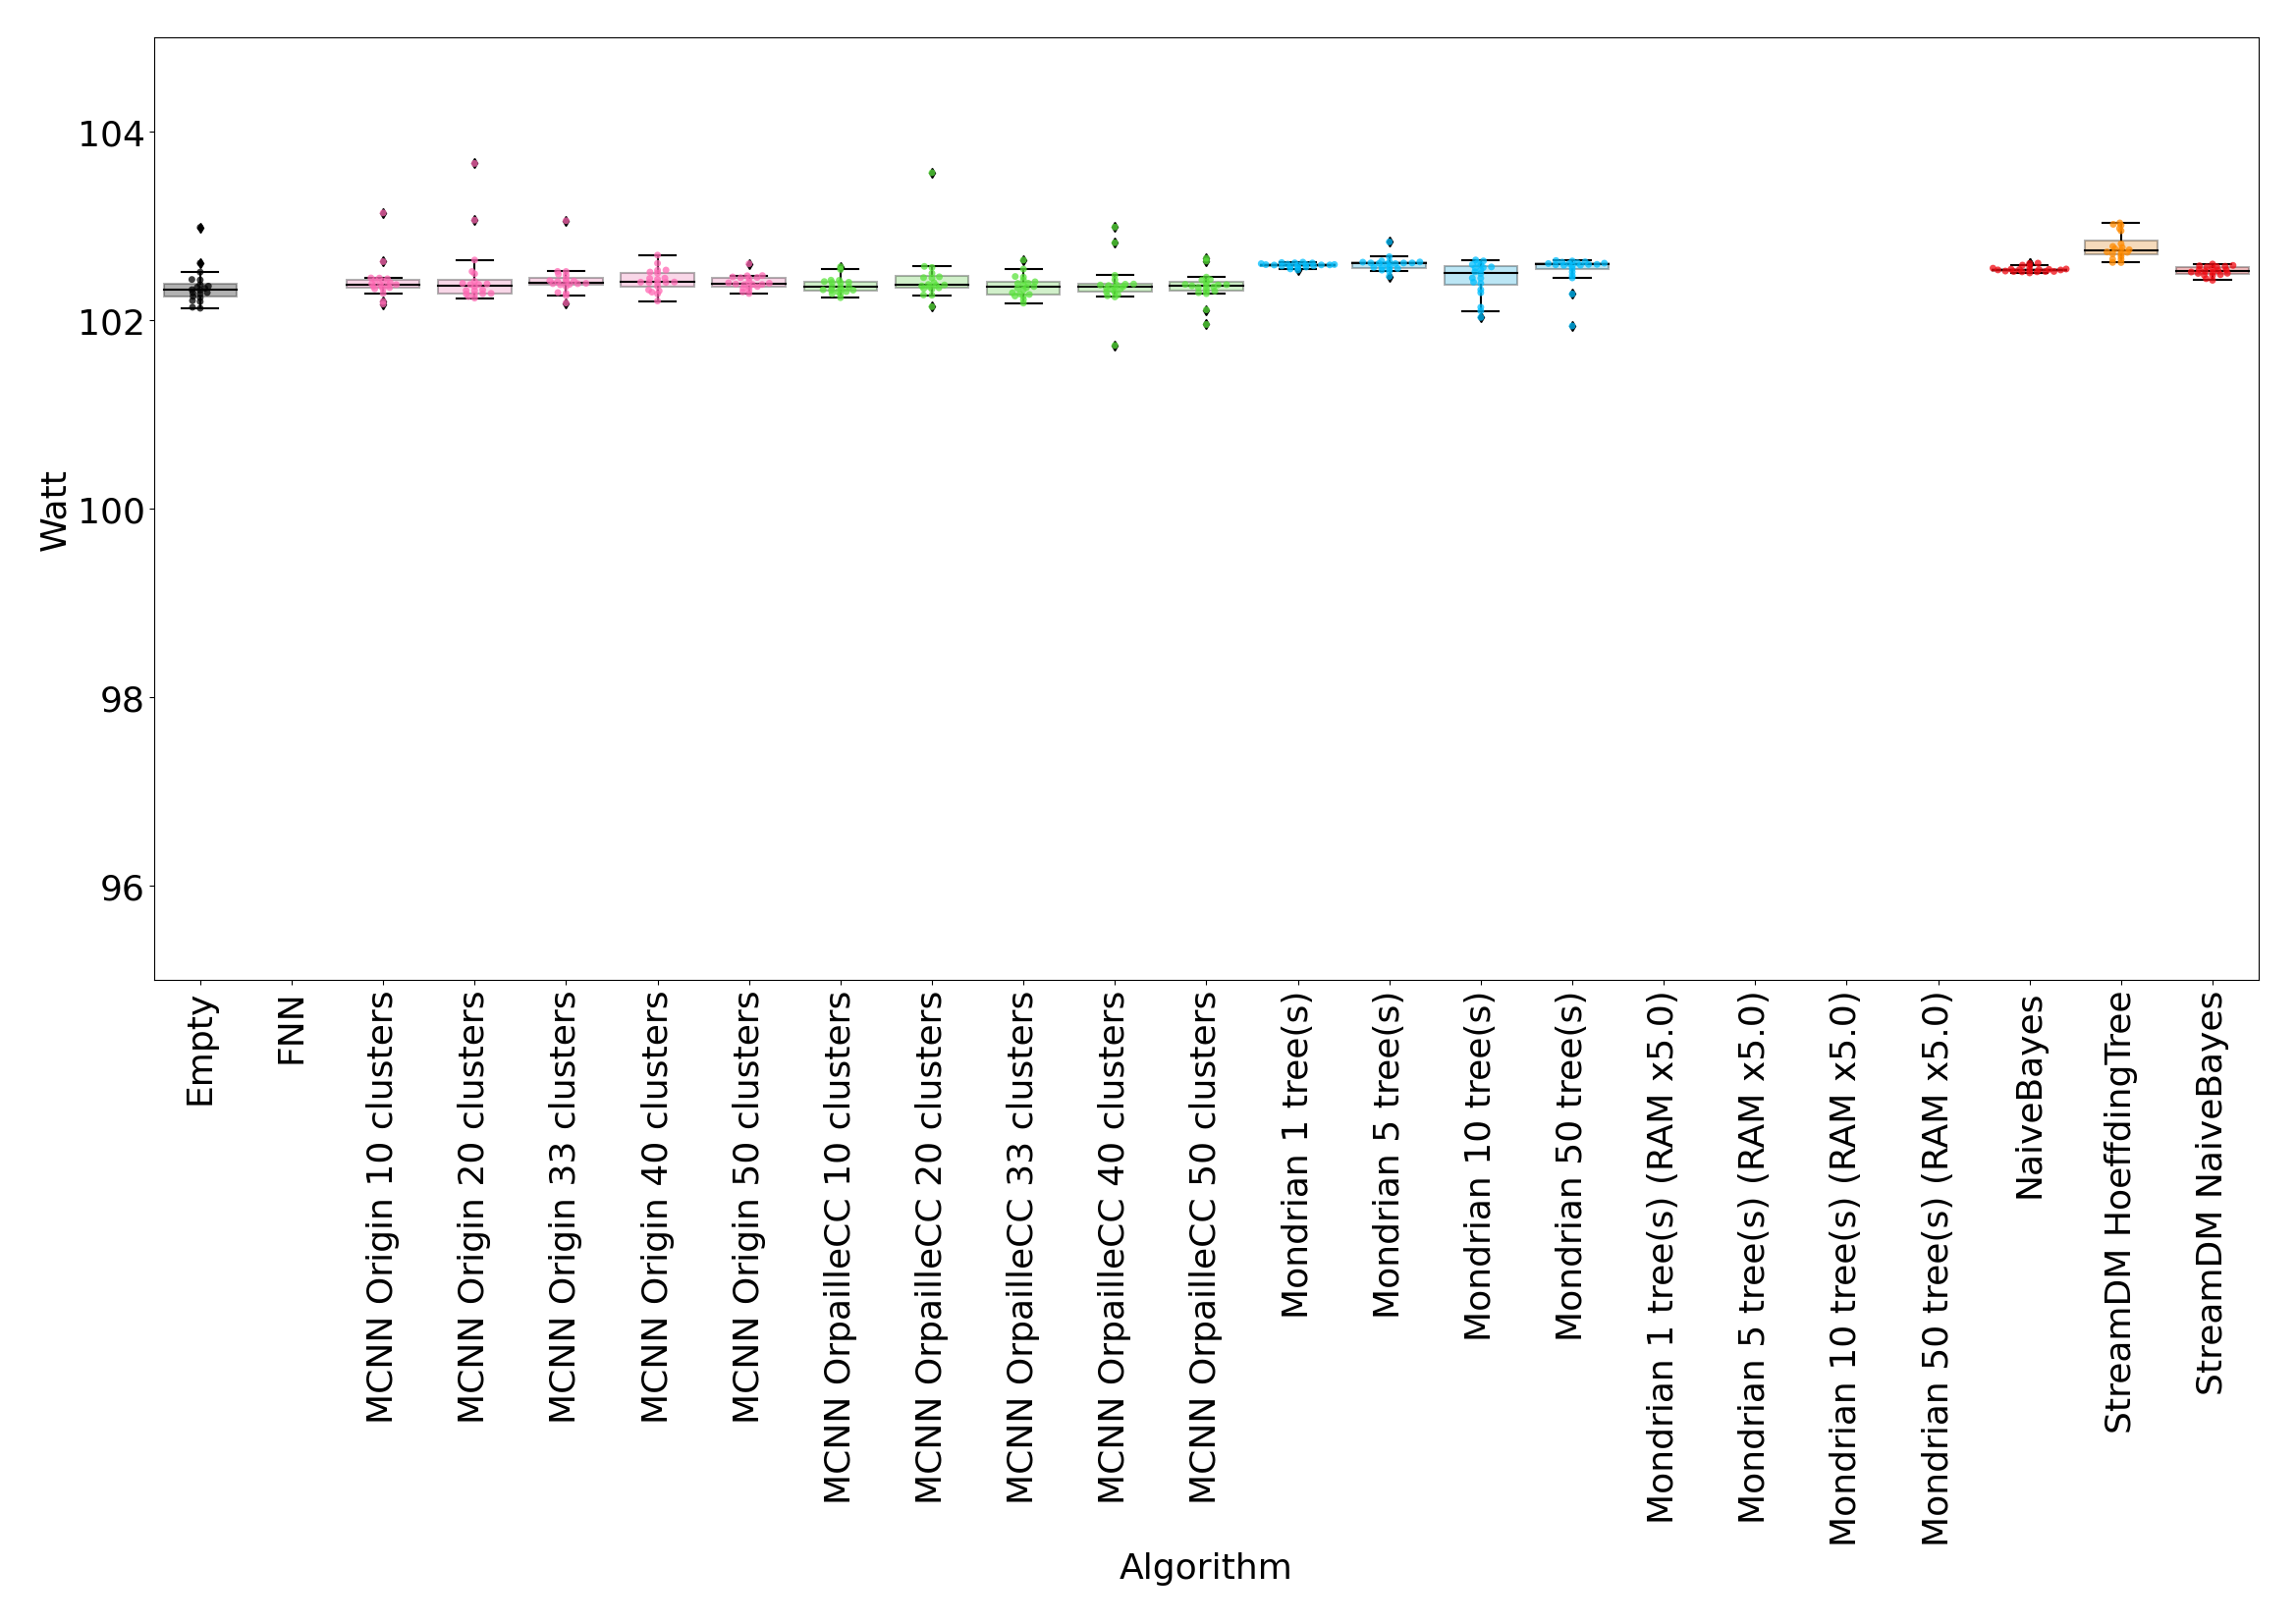
\includegraphics[width=\linewidth]{figures/results/recofit_3_watt.png}
		\caption{\recofitdataset}
		\label{fig:power-recofit}
	\end{subfigure}
	\begin{subfigure}[t]{.5\linewidth}
		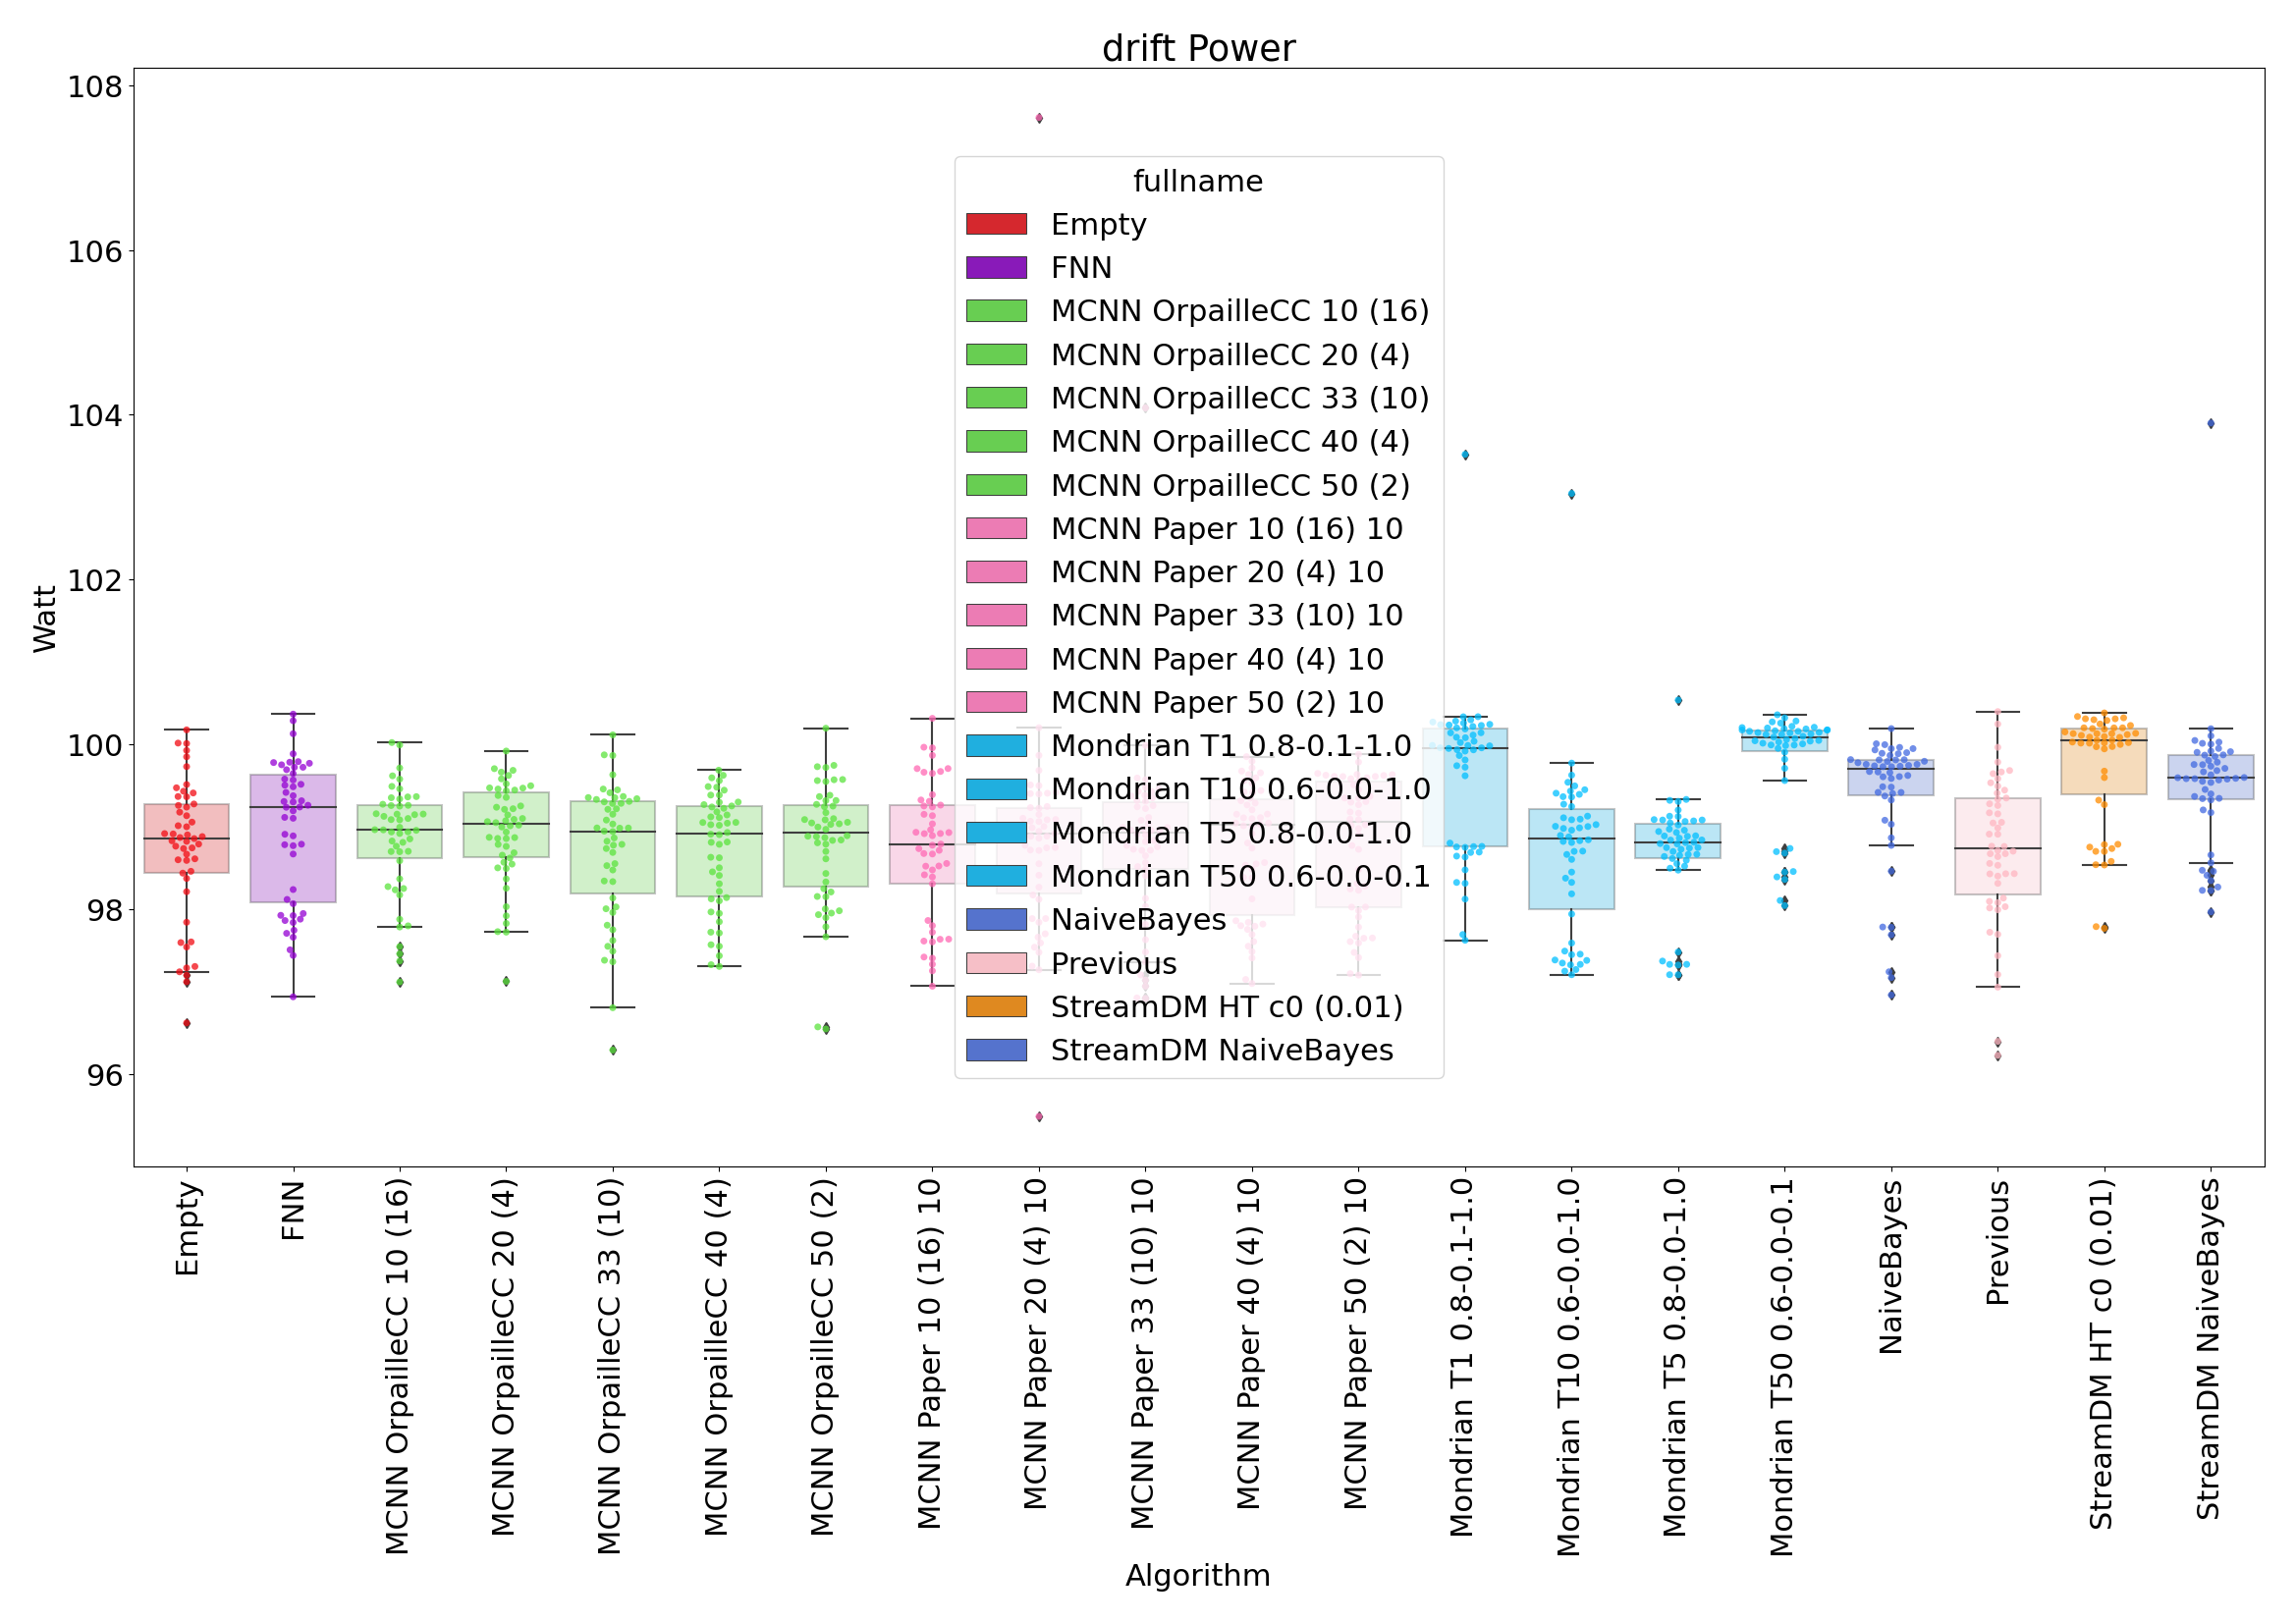
\includegraphics[width=\linewidth]{figures/results/drift_watt.png}
		\caption{\banosdataset with drift.}
		\label{fig:power-drift}
	\end{subfigure}
	\begin{subfigure}[t]{.5\linewidth}
		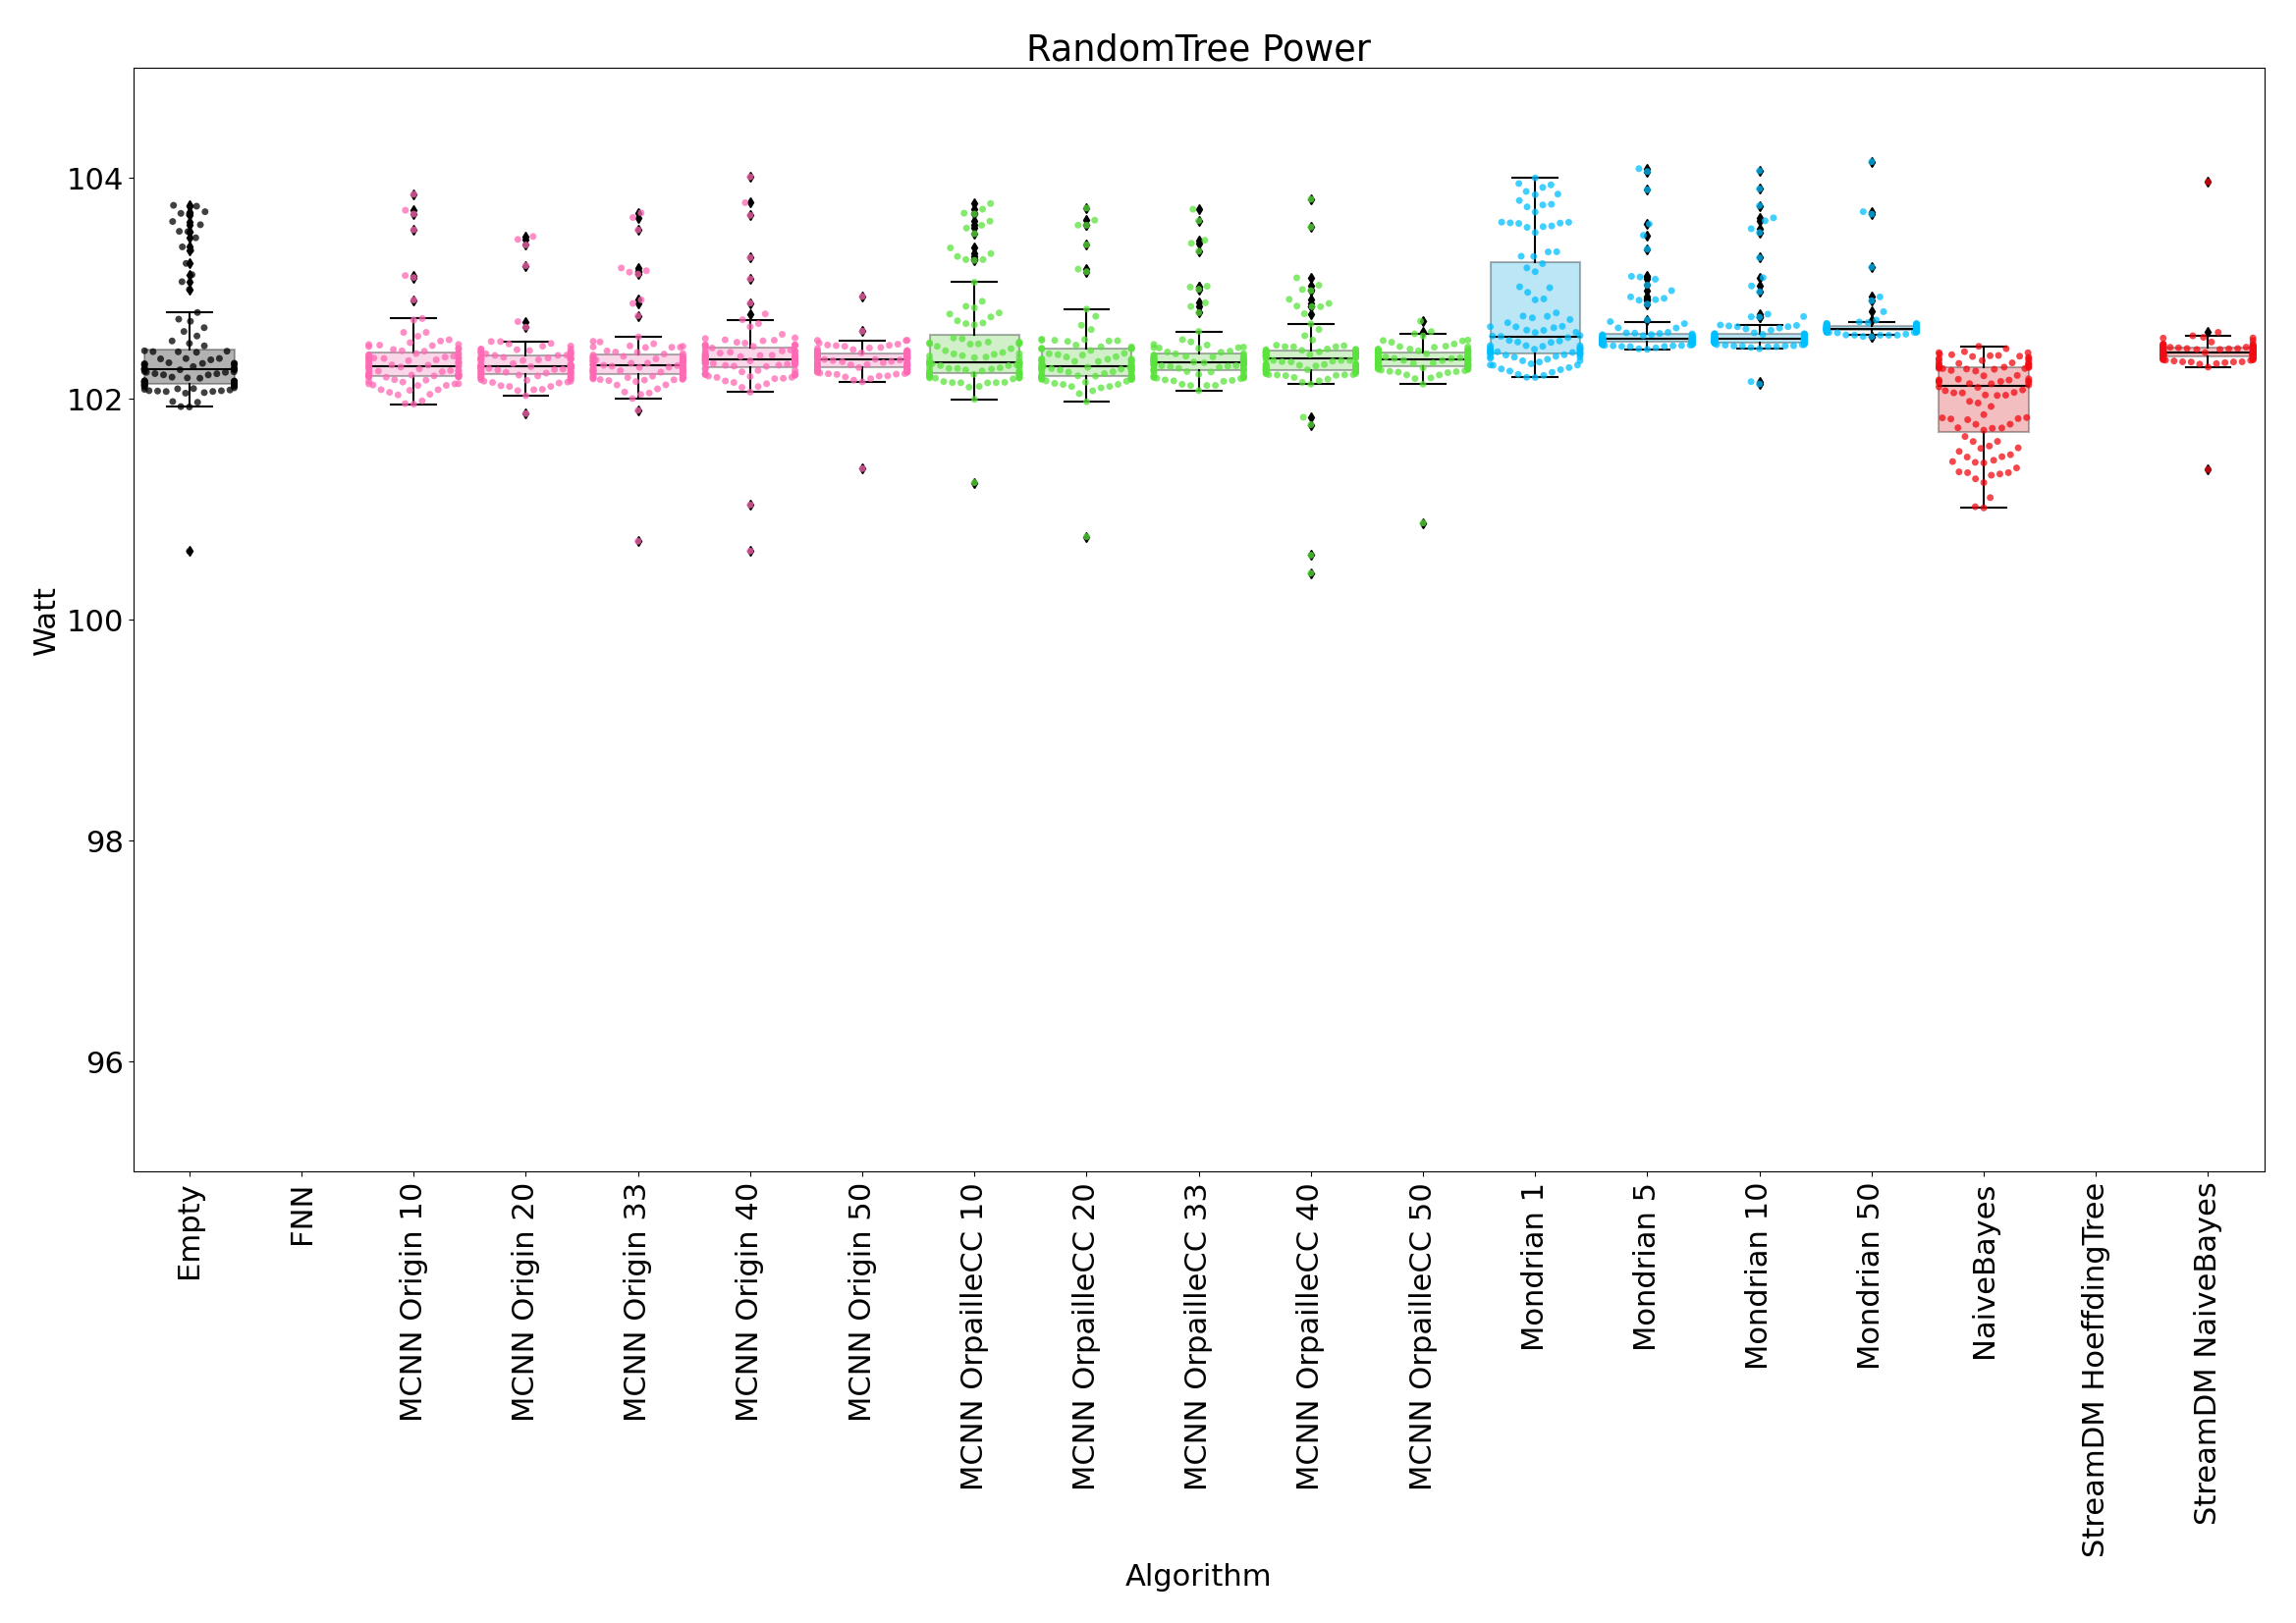
\includegraphics[width=\linewidth]{figures/results/dataset_3_watt.png}
		\caption{RandomTree}
		\label{fig:power-dataset_3}
	\end{subfigure}
	\caption{Power usage on four datasets.}
	\label{fig:power}
\end{figure*}

\subsection{Runtime}
Figure~\ref{fig:runtime} shows the runtime results on two datasets:
\banosdataset and \recofitdataset. We observe that the Mondrian algorithm is
the slowest especially with high a number of trees.
It is then followed by the HoeffdingTree. Depending on the dataset, the
HoeffdingTree tree can take more time than Mondrian with 10 trees or take as
much time as Mondrian with 1 tree.

The HoeffdingTree is followed by the two naïve Bayes which are systematically
faster.  This can be explained by the naïve Bayes classifiers that run in the HoeffdingTree
leaves, so the HoeffdingTree takes at least as much time as a naïve Bayes.

We observe that naïve Bayes from StreamDM is slightly faster than the one from
OrpailleCC.

Finally, the MCNNs are the fastest and they are barely noticeable compared to an
empty classifier. There is still a slight difference between the MCNNs. The
more cluster we use, the slower it gets.

\begin{figure*}
	\begin{subfigure}[t]{.5\linewidth}
		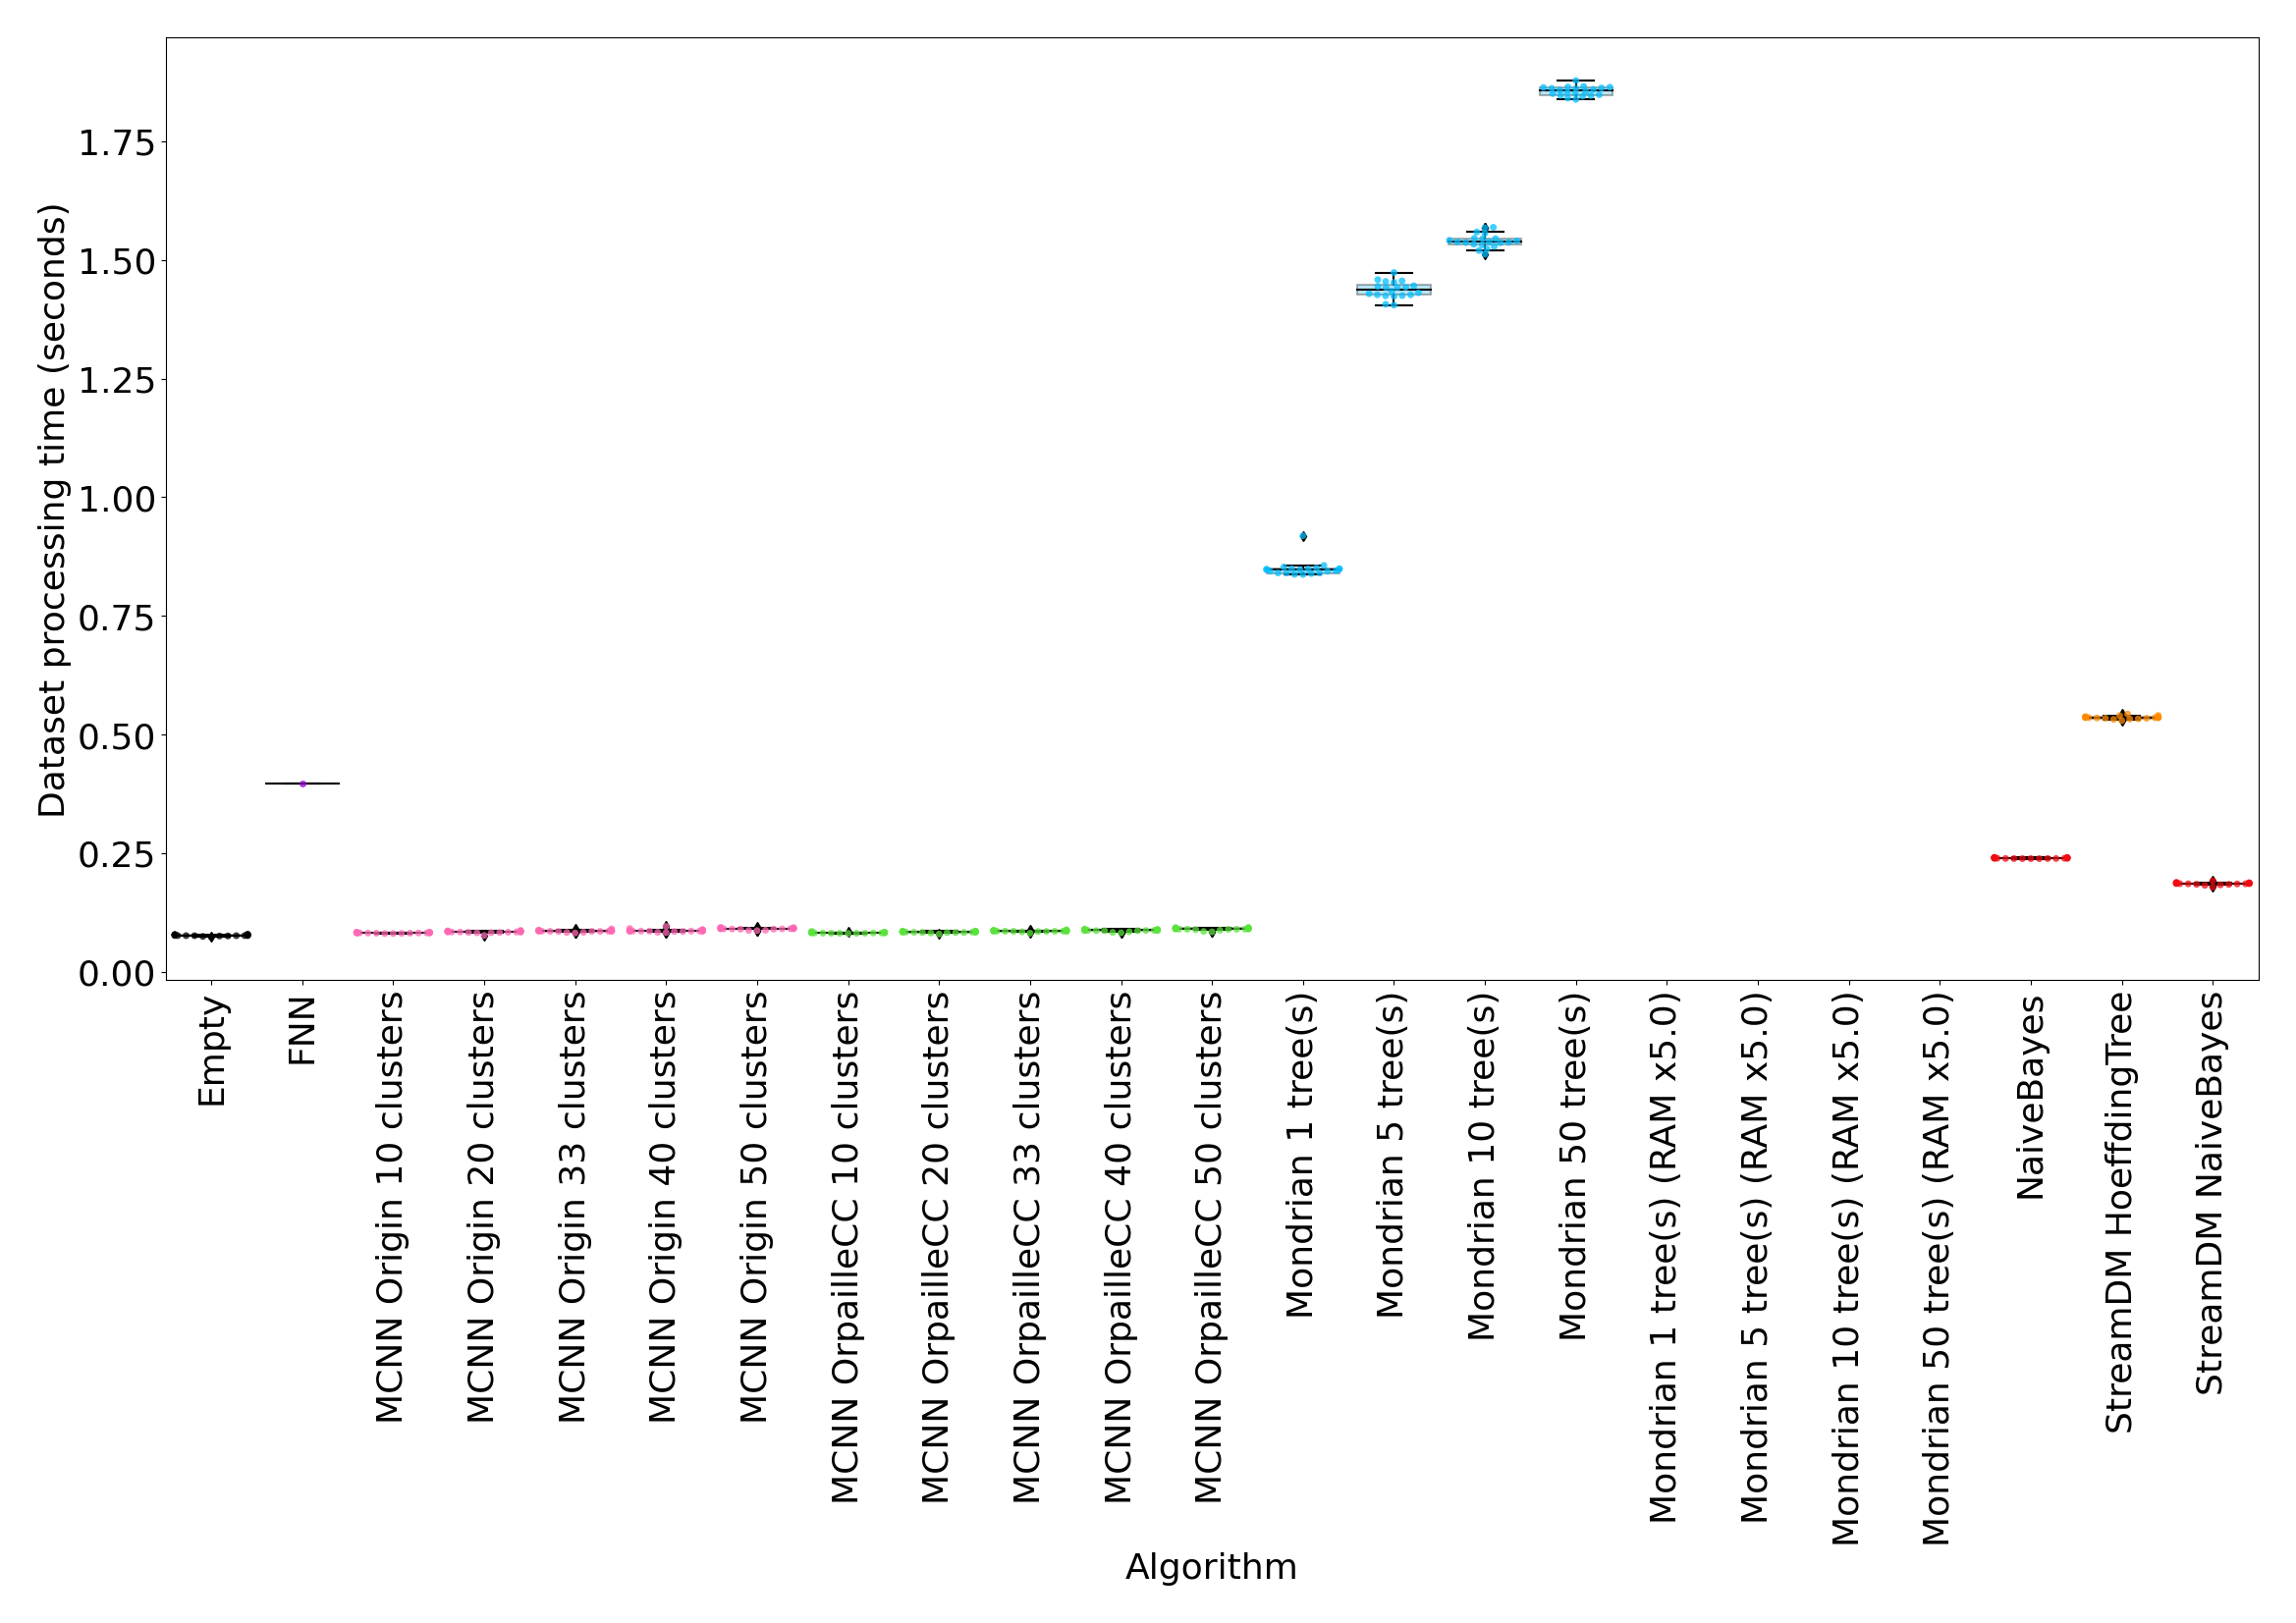
\includegraphics[width=\linewidth]{figures/results/banos_3_runtime.png}
		\caption{\banosdataset}
		\label{fig:runtime-banos}
	\end{subfigure}
	\begin{subfigure}[t]{.5\linewidth}
		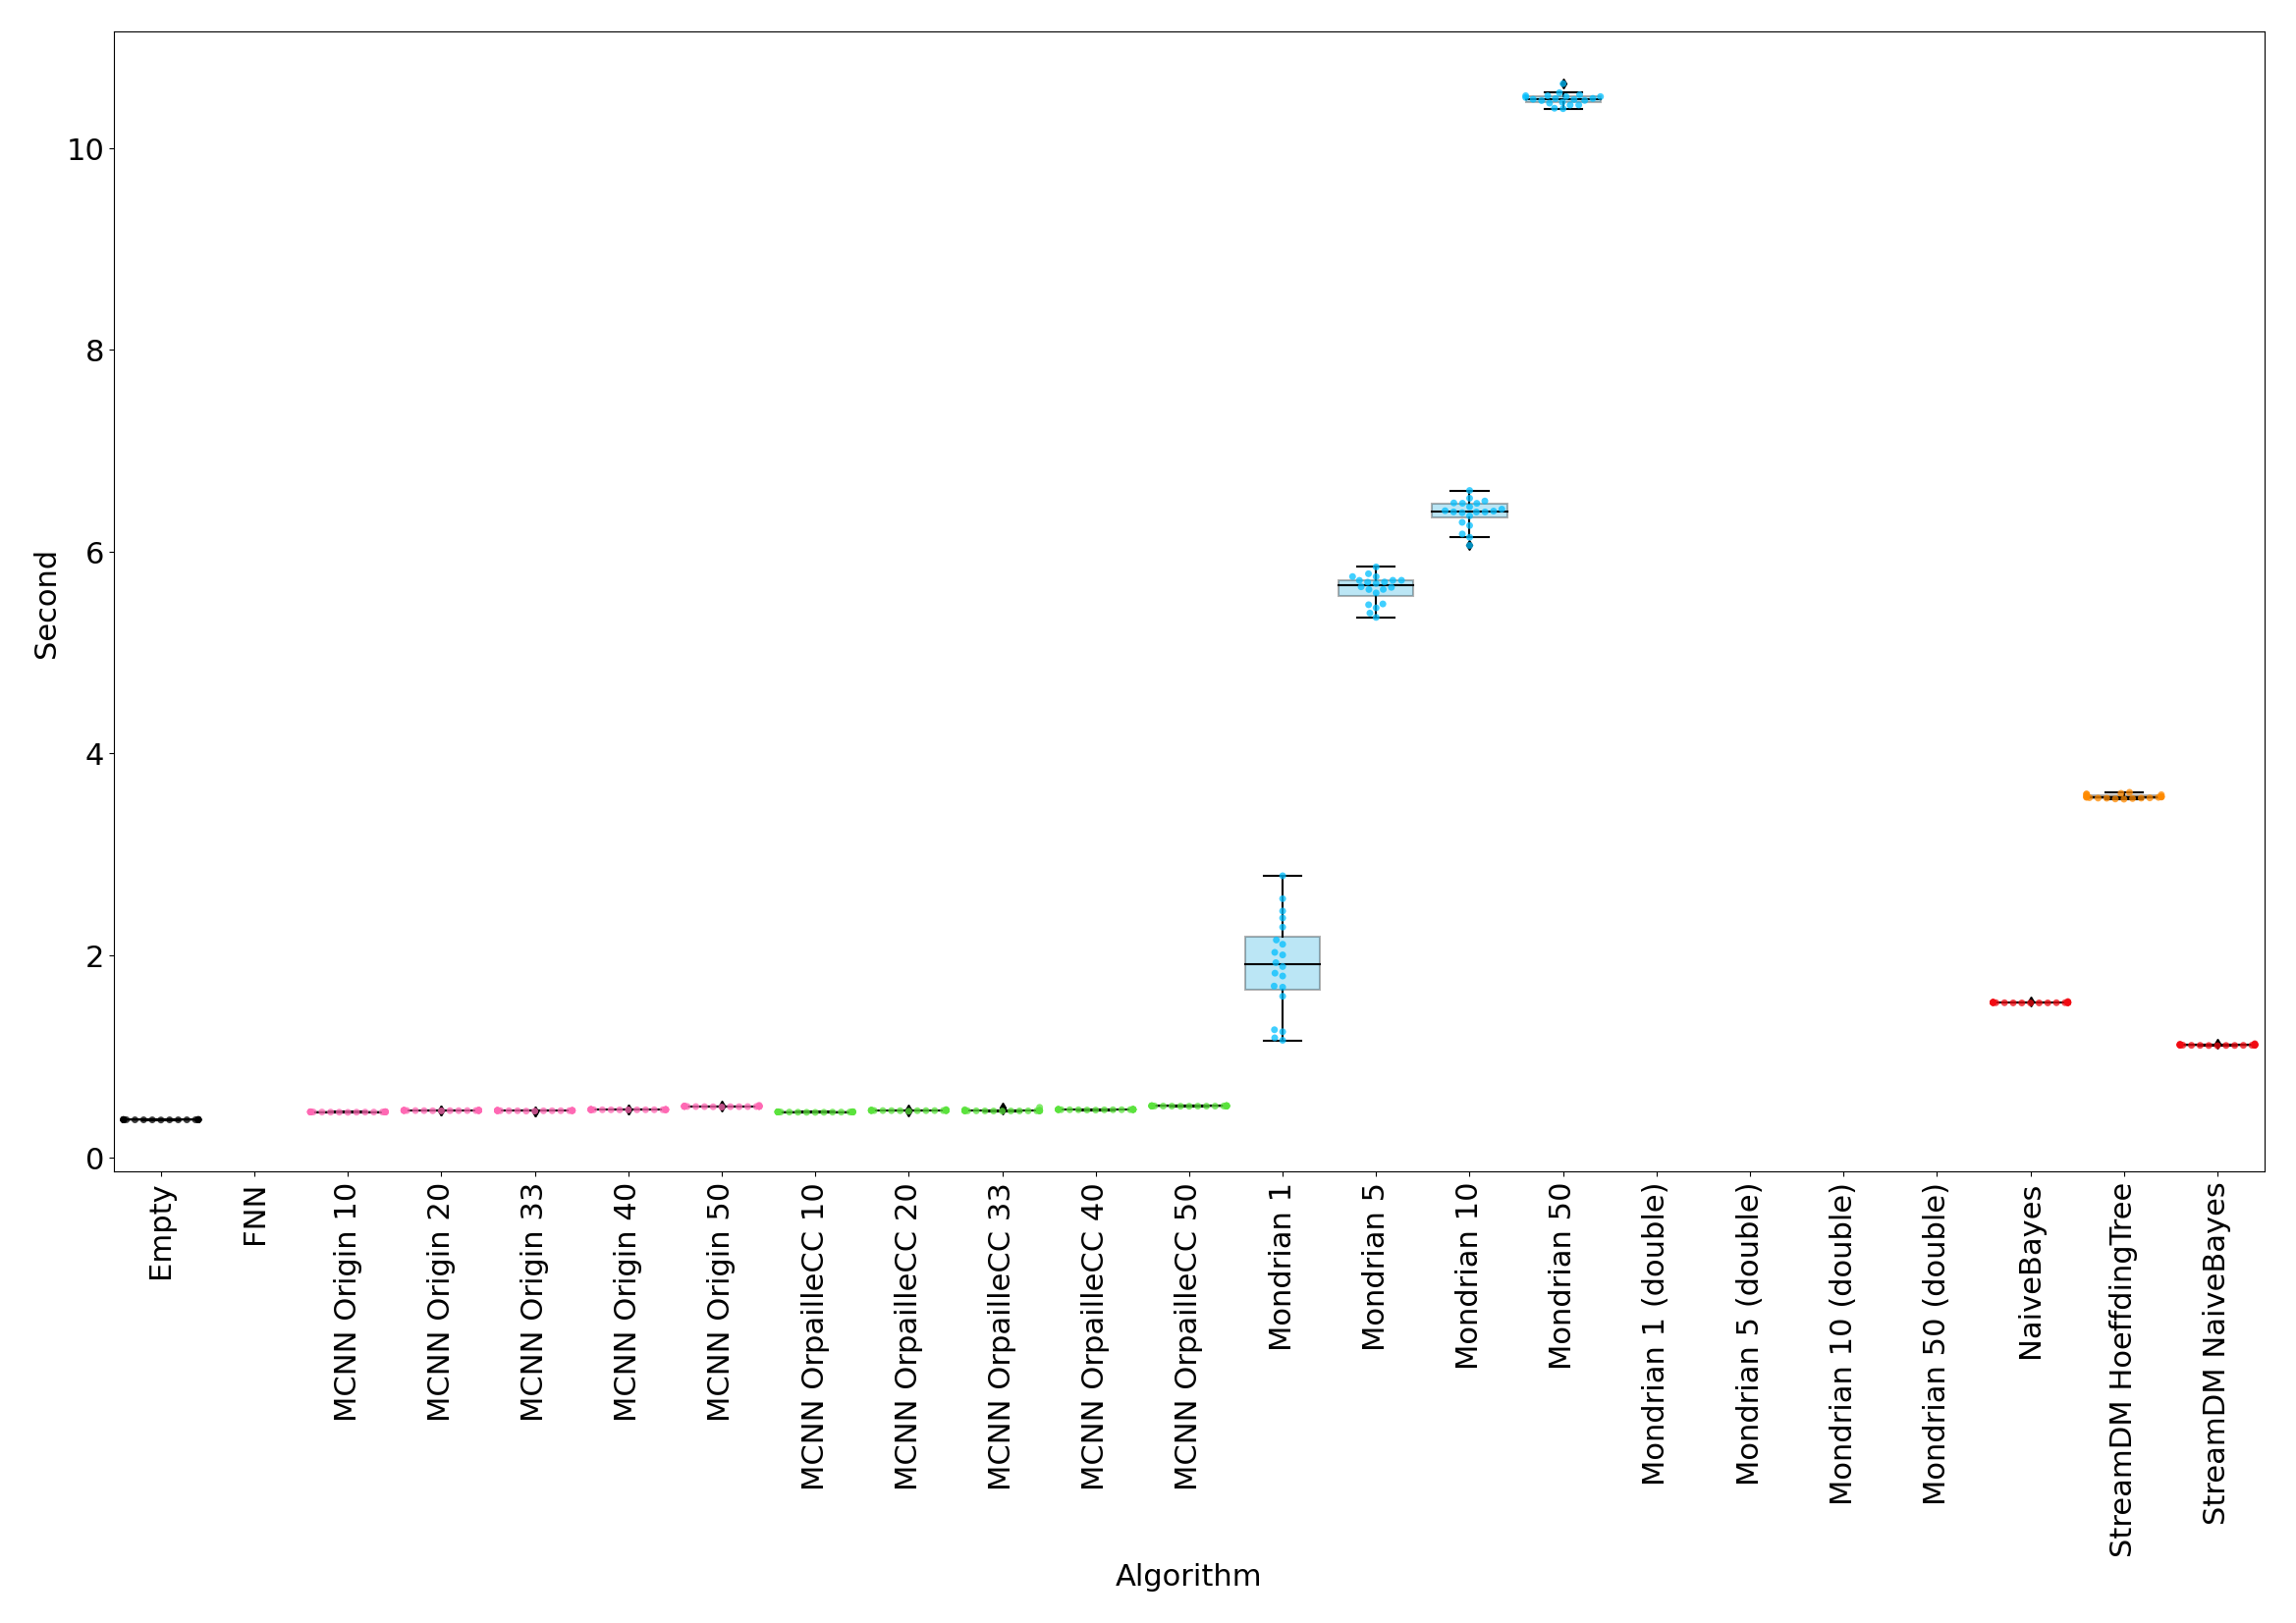
\includegraphics[width=\linewidth]{figures/results/recofit_3_runtime.png}
		\caption{\recofitdataset}
		\label{fig:runtime-recofit}
	\end{subfigure}
	\caption{Runtime with the two real datasets.}
	\label{fig:runtime}
\end{figure*}

\subsection{Memory}
\label{sec:result-memory}
Figure~\ref{fig:memory} shows the evolution of the memory footprint for the
\banosdataset.  It is similar across all datasets because most algorithms
follow a bounded memory policy or have a constant space complexity. The only
exception is the HoeffdingTree that constantly selects new splits in regard to
the new data. Note that the Mondrian would have had the same behavior if it
would allocate memory as element goes by. However, the Mondrian implementation
of OrpailleCC allocates memory when the classifier is instantiated and does not
use more.

\begin{figure}[H]
	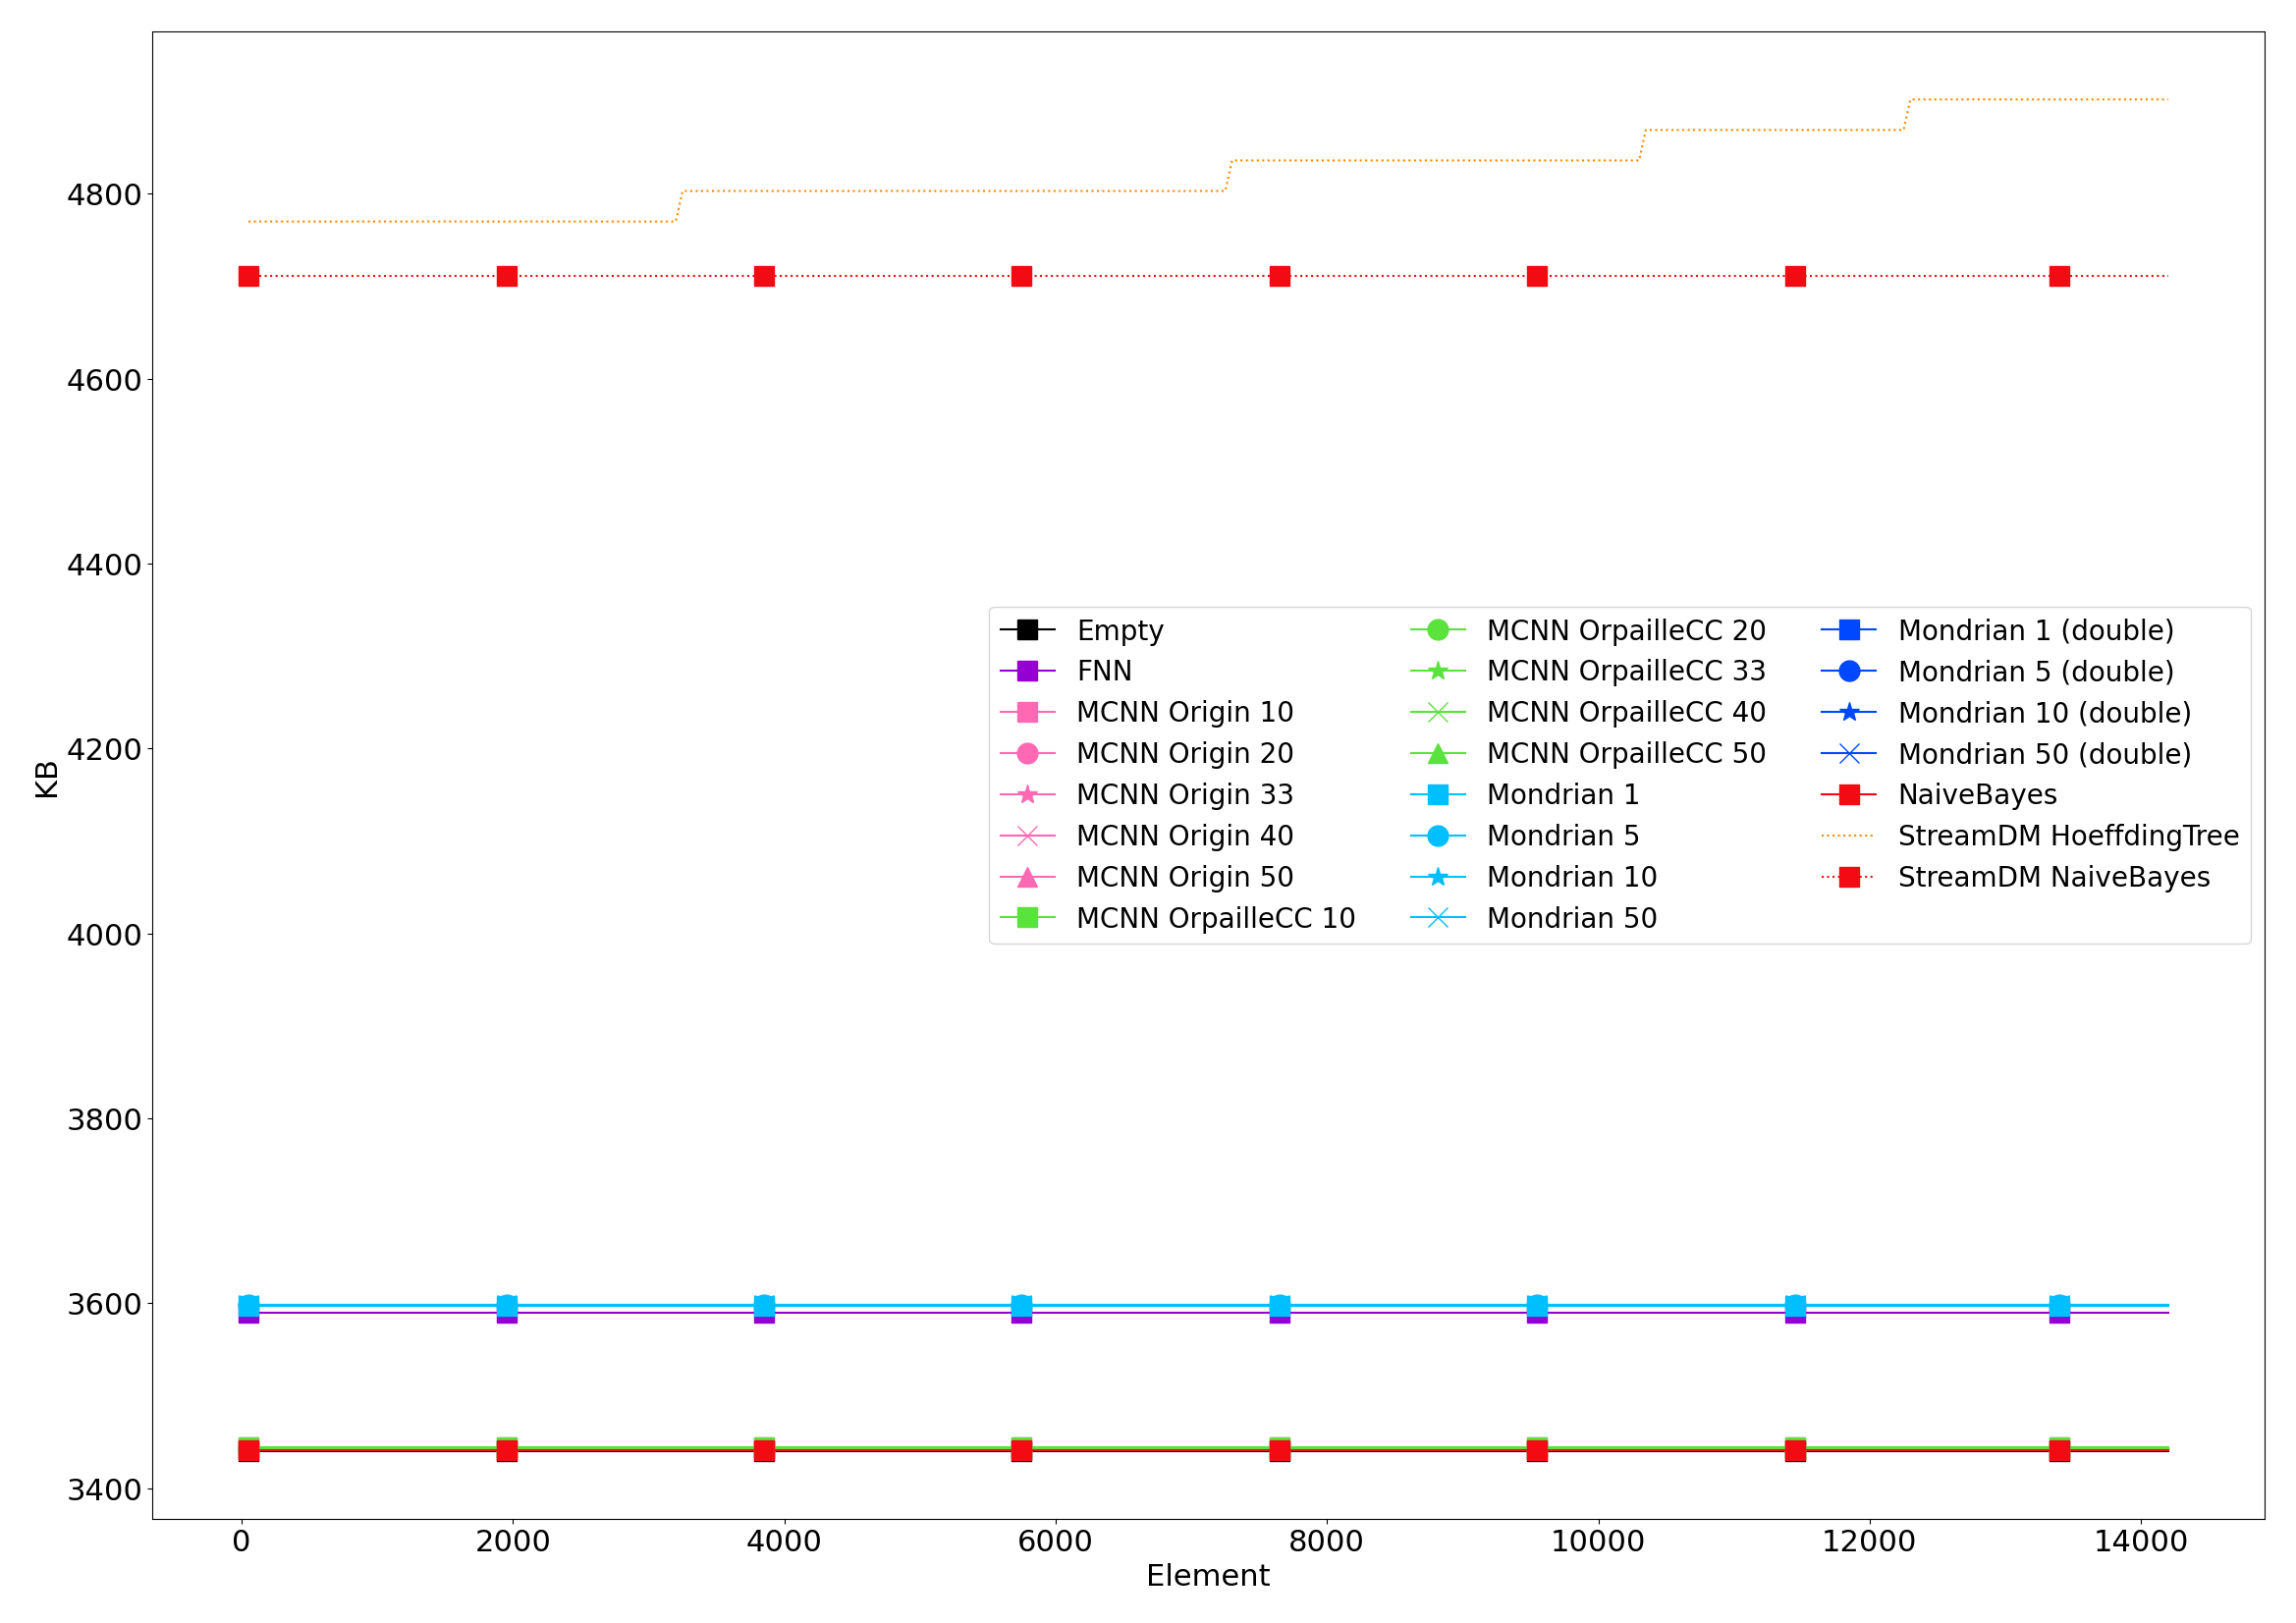
\includegraphics[width=\linewidth]{figures/results/banos_3_memory.png}
	\caption{Memory used by the algorithms on the Banos dataset.}
	\label{fig:memory}
\end{figure}


\subsection{Micro-Cluster Nearest Neighbor tuning}
Figure~\ref{fig:mcnn-tuning-error} shows the impact of the error threshold with
different numbers of clusters. On this figure, we observe that the higher the
cluster count is, the better are the performance. We also observe that the
error threshold of MCNN has little impact on these classification performances.
The best threshold to use is either 2 or 4 which means that a cluster may do 2
or 4 error before being split in two.
However, we note that it does not apply with 10 clusters only where the
plots are indistinguishable.

\begin{figure}[H]
	 \begin{subfigure}[b]{0.49\textwidth}
		 \centering
		 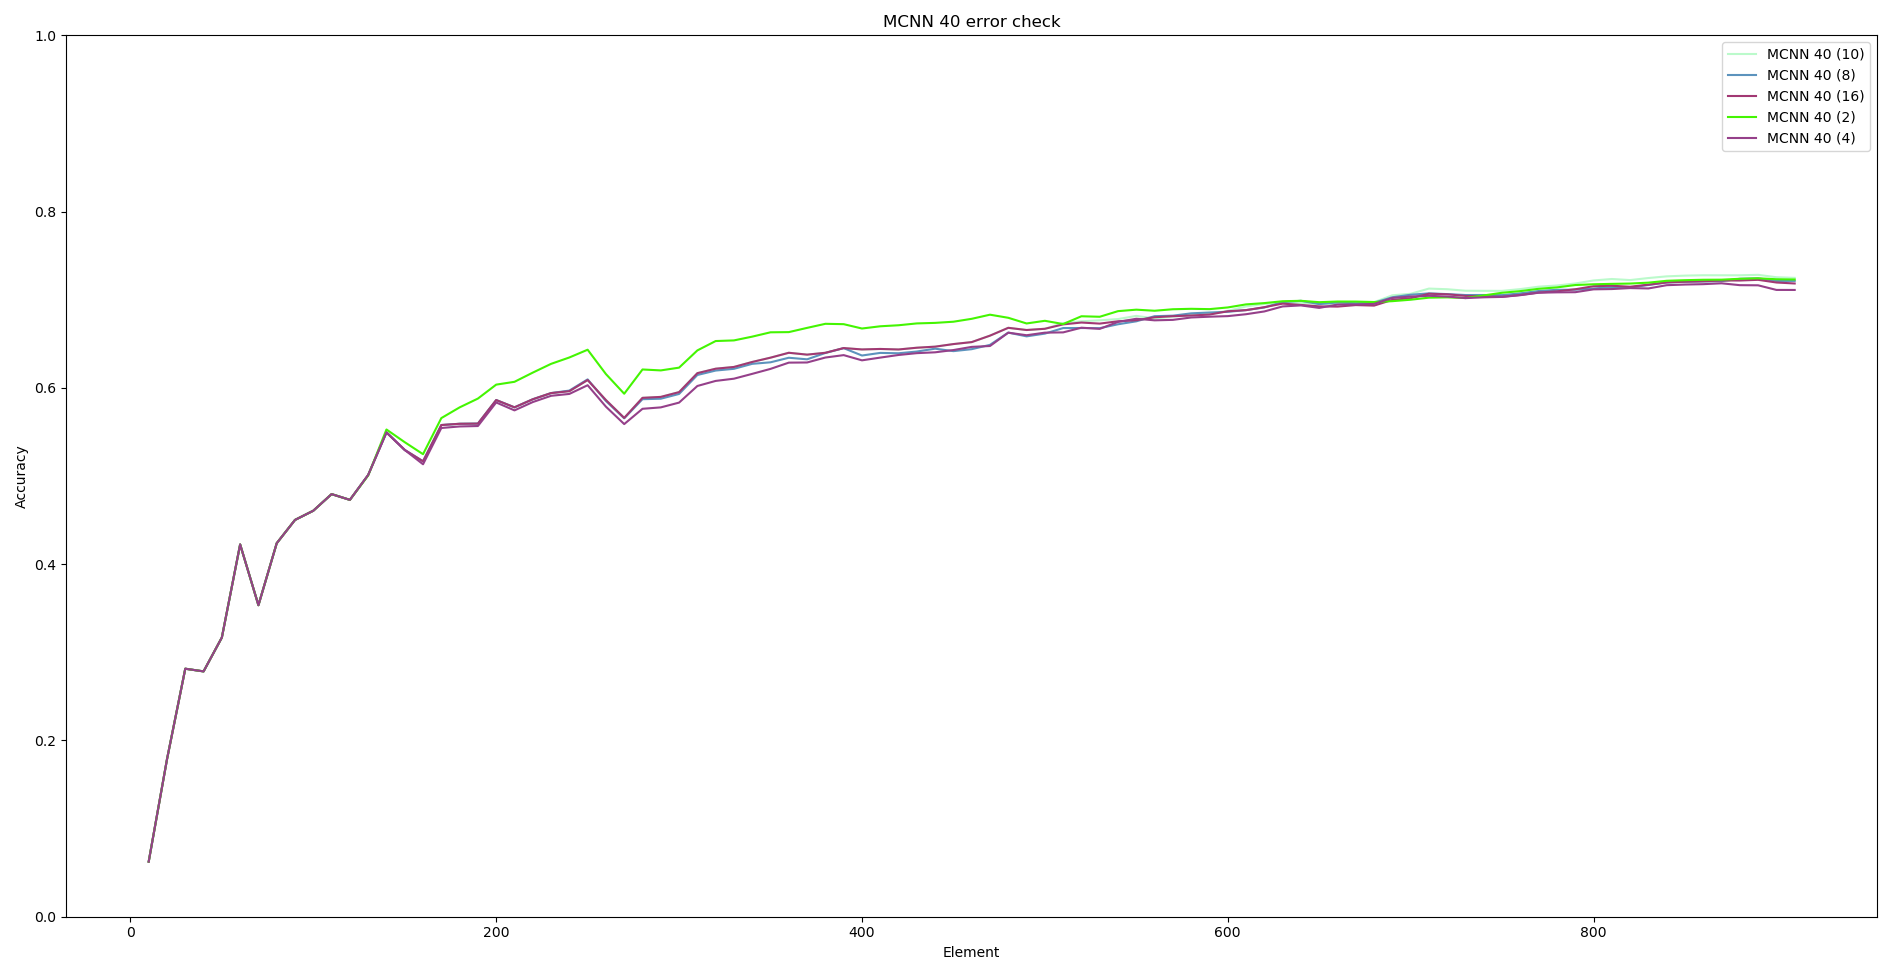
\includegraphics[width=\linewidth]{figures/Banos_S1_shuf_MCNN_40_error_check.png}
		 \caption{40 clusters}
	 \end{subfigure}
	 \begin{subfigure}[b]{0.49\textwidth}
		 \centering
		 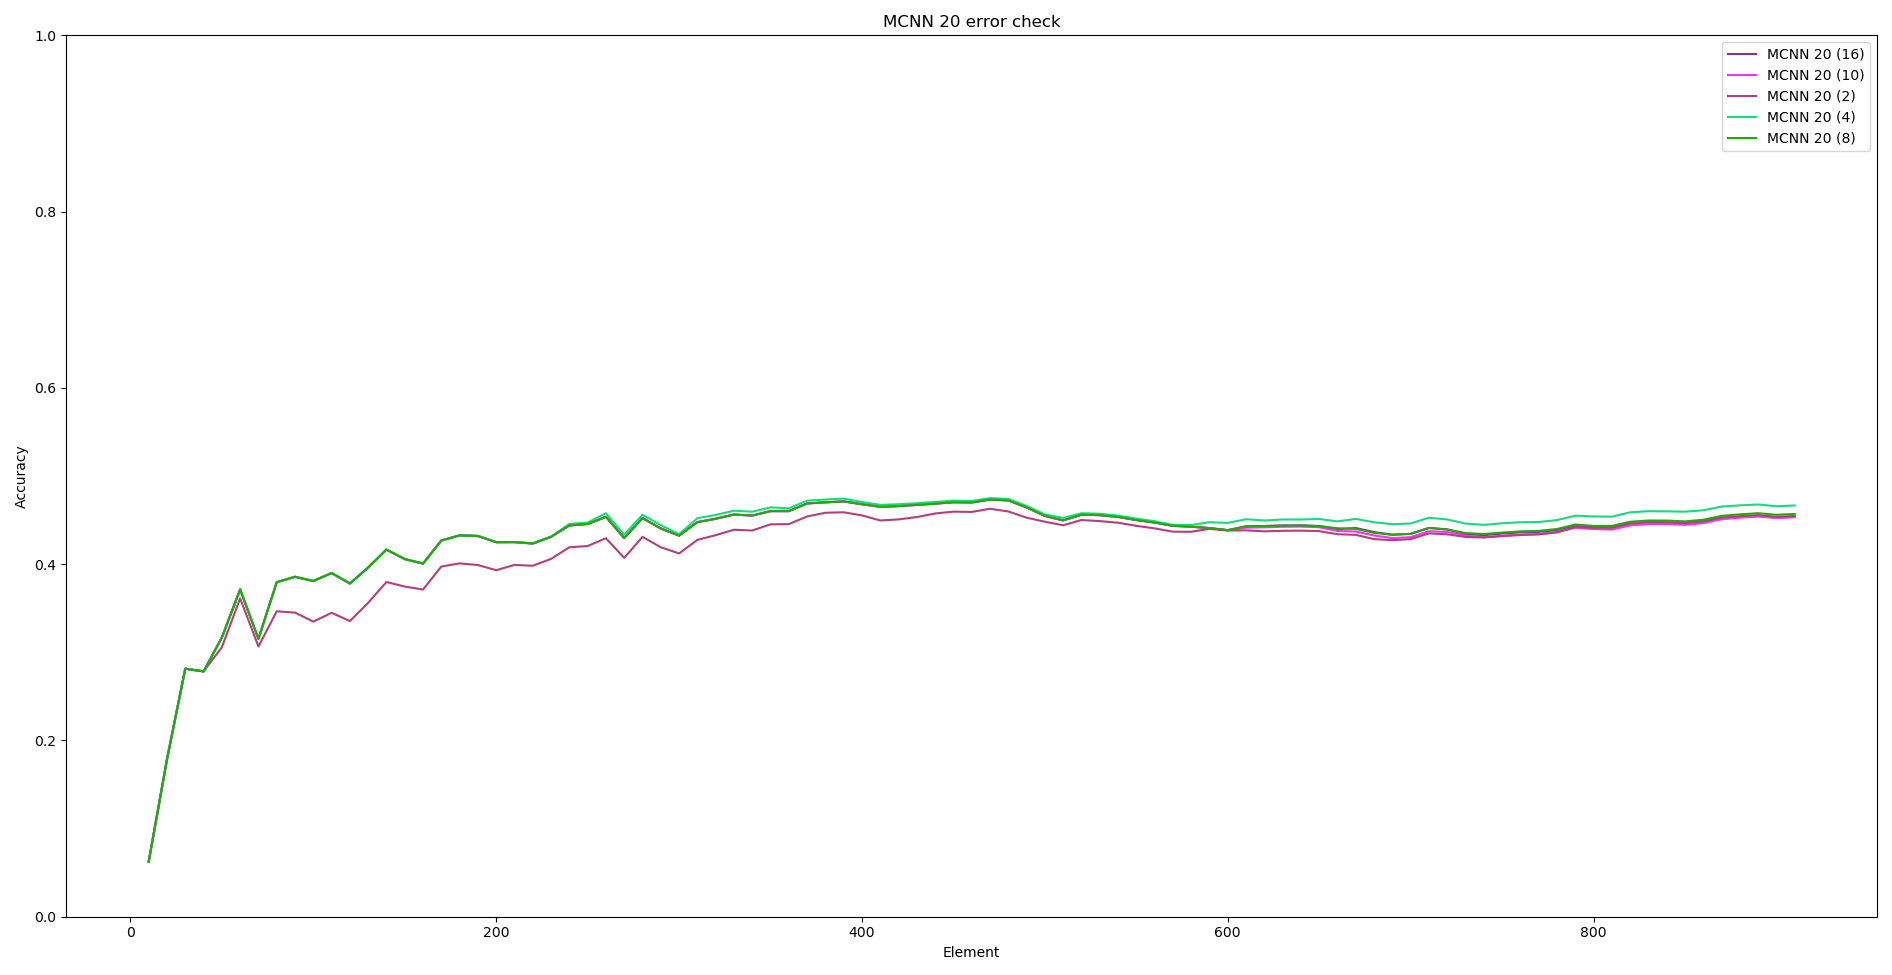
\includegraphics[width=\linewidth]{figures/Banos_S1_shuf_MCNN_20_error_check.png}
		 \caption{20 clusters}
	 \end{subfigure}
	 \begin{subfigure}[b]{0.49\textwidth}
		 \centering
		 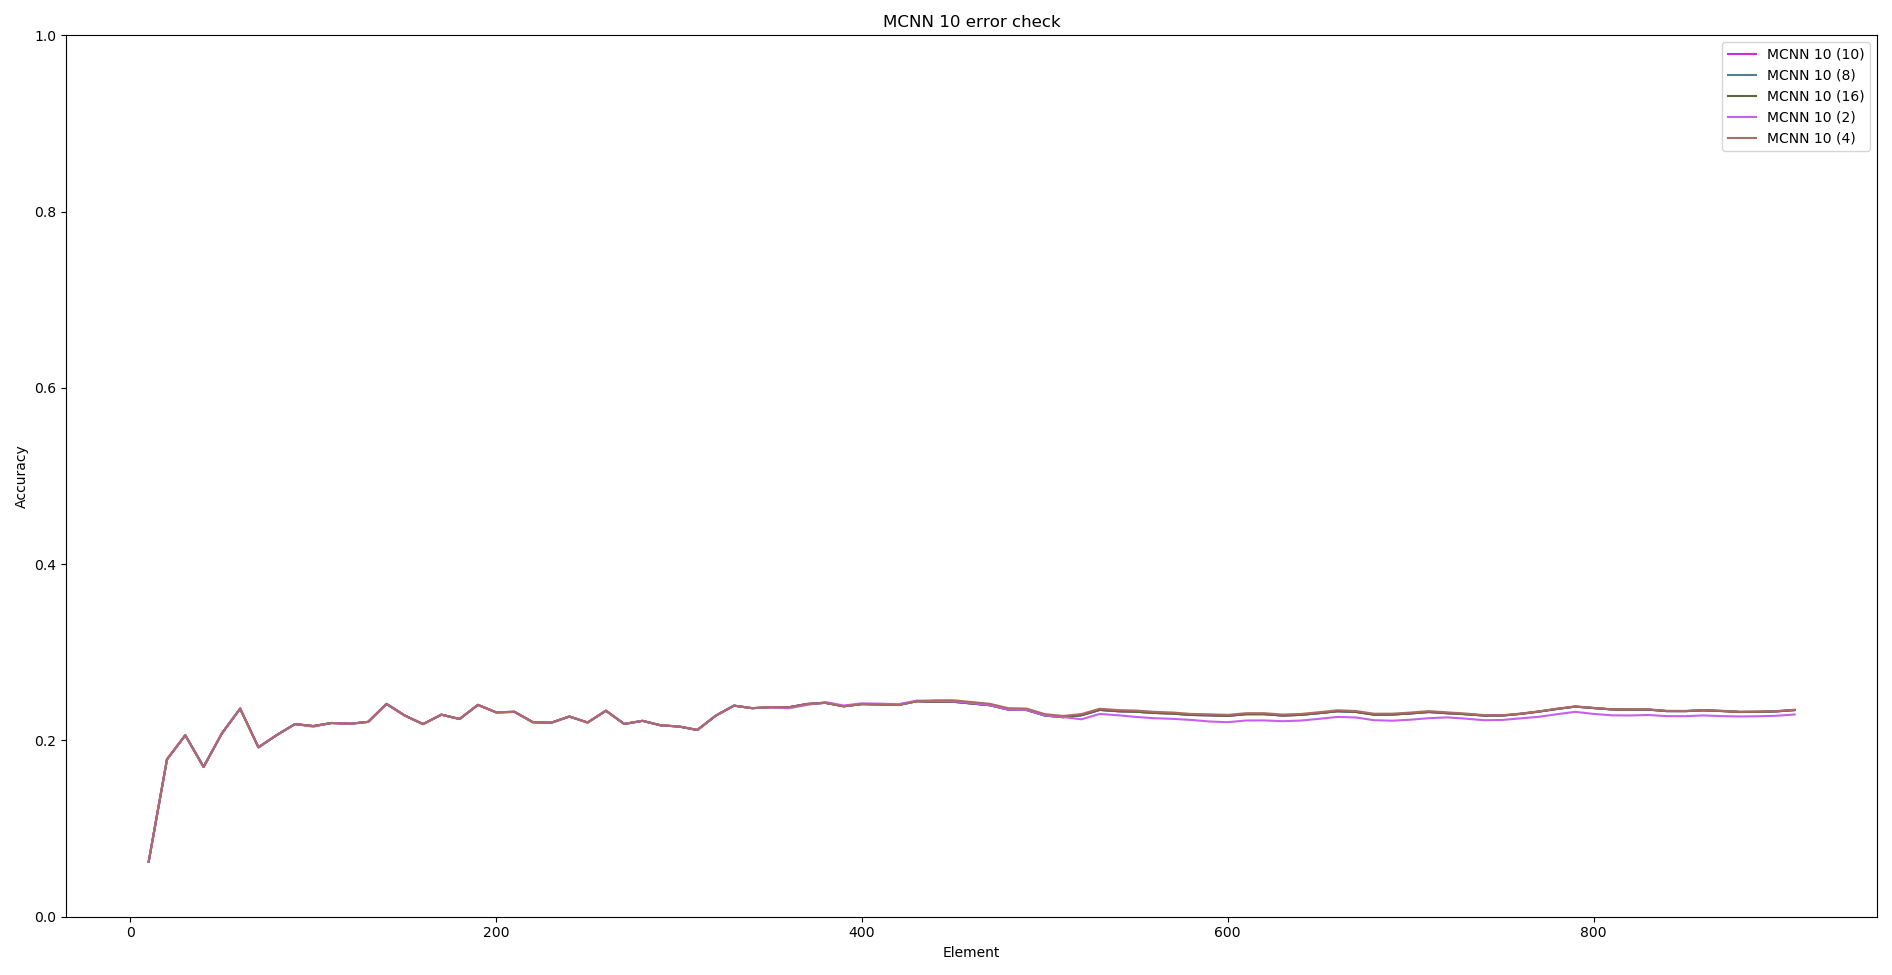
\includegraphics[width=\linewidth]{figures/Banos_S1_shuf_MCNN_10_error_check.png}
		 \caption{10 clusters}
	 \end{subfigure}
	\caption{Impact of the error threshold on MCNN.}
	\label{fig:mcnn-tuning-error}
\end{figure}

\subsection{Mondrian Tuning}
Figure~\ref{fig:mondrian-tuning} shows the impact of the Mondrian parameters on
the classification performances. Occasionally, dashed lines are used to
emphasize the minimum and the maximum.

Figure~\ref{fig:mondrian-budget} shows the impact of the budget parameter. We
see that this parameter induces a slight impact as the lines are packed
together. We note that the best budget for 10 trees is slightly below 1.0. 

Figure~\ref{fig:mondrian-base-count} shows the impact of the base count
parameter. We observe a huge impact of this parameter on the classification
performances. We note that the smallest values of the base count present the
best performances.

Finally, Figure~\ref{fig:mondrian-discount} exhibits the small impact of the
discount parameter. Indeed, the figure is zoomed on one specific area and the
accuracy difference between the minimum and the maximum is 0.01. However,
despite the indistinguishable impact, we note that the best value for this
parameter is 0.1.

\begin{figure}
	 \centering
	 \begin{subfigure}[b]{0.49\textwidth}
		 \centering
		 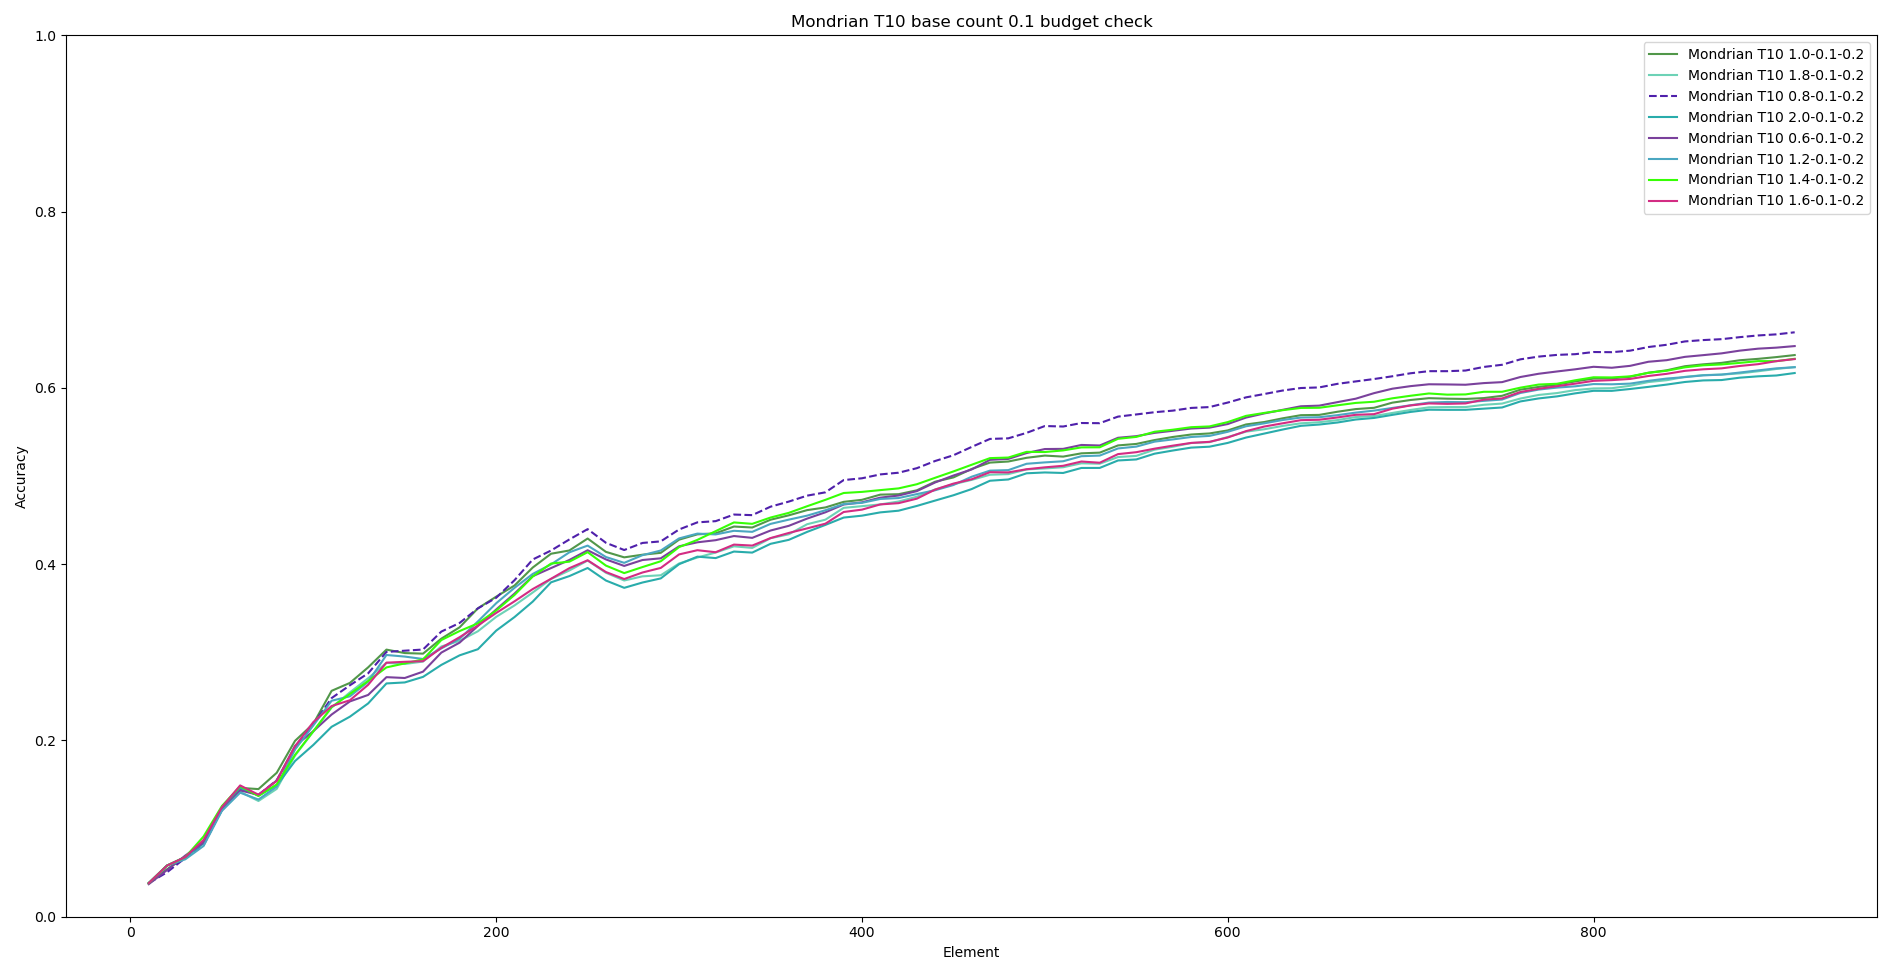
\includegraphics[width=\textwidth]{figures/Banos_S1_shuf_Mondrian_T10_bc_0.1_budget_check.png}
		 \caption{Impact of the budget with 10 trees, a base count of $0.1$, and discount factor of $0.2$.}
		 \label{fig:mondrian-budget}
	 \end{subfigure}
	 \hfill
	 \begin{subfigure}[b]{0.49\textwidth}
		 \centering
		 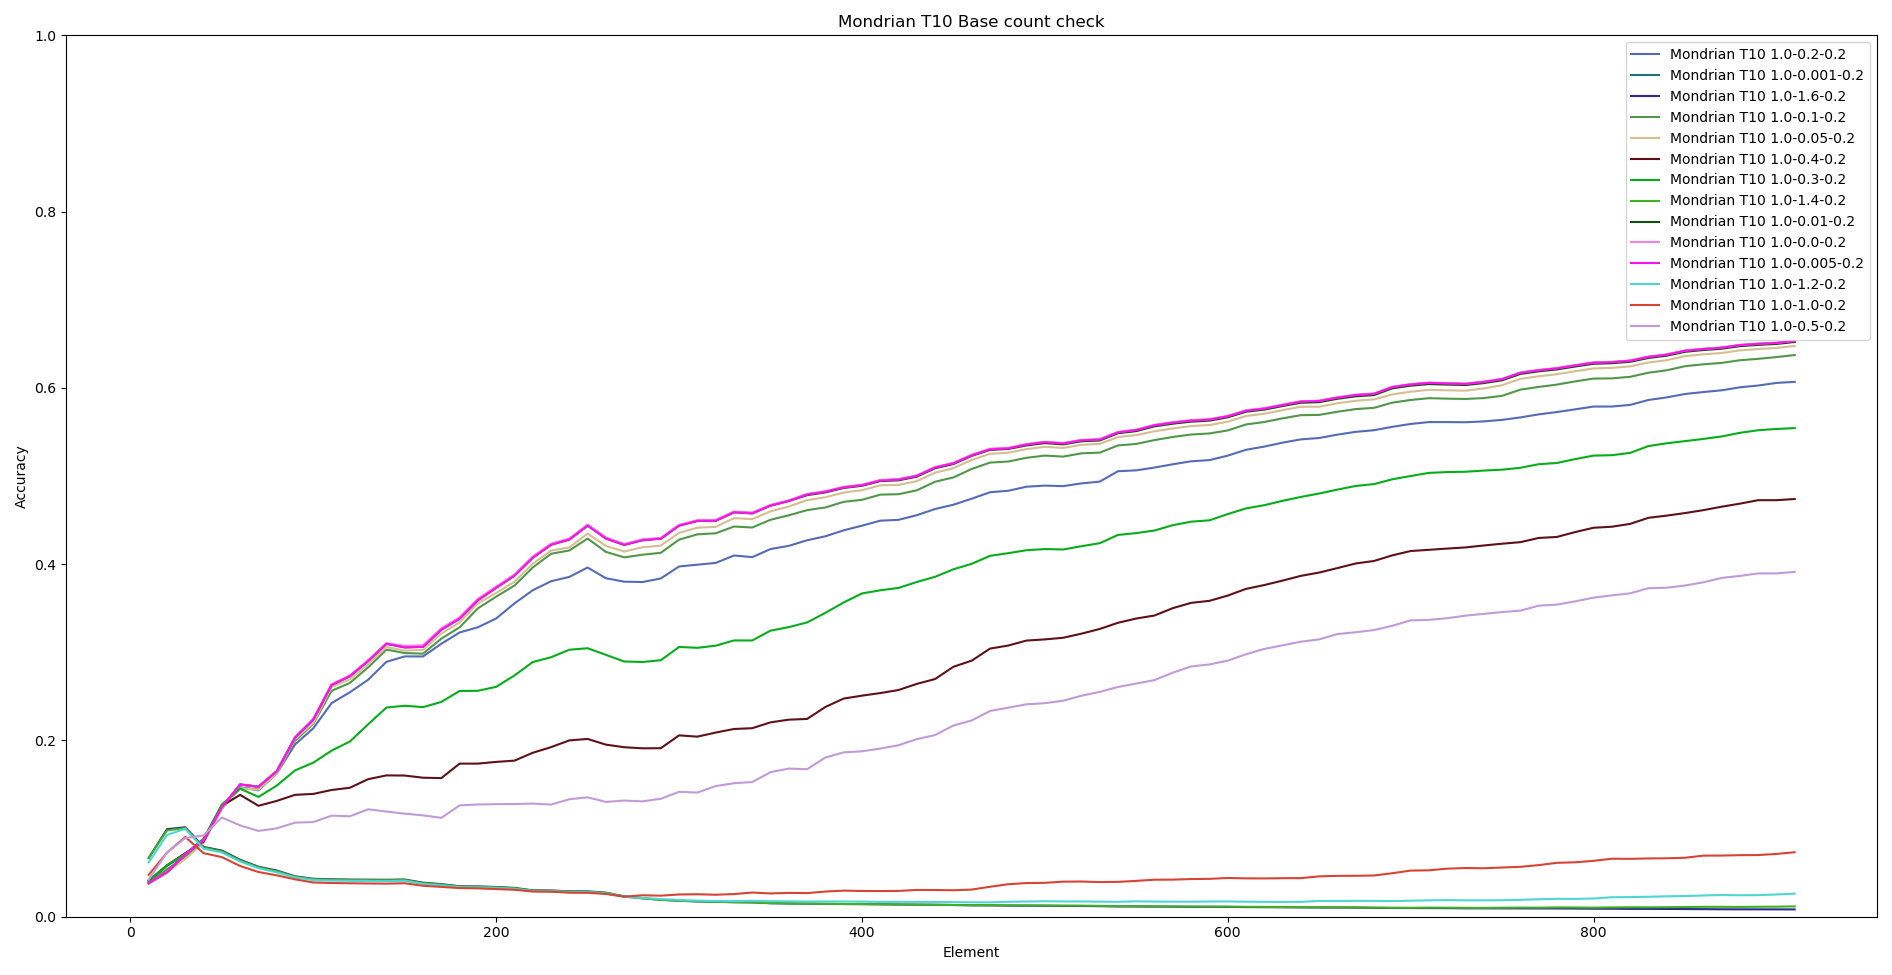
\includegraphics[width=\textwidth]{figures/Banos_S1_shuf_Mondrian_T10_check.png}
		 \caption{Impact of the base count with 10 trees, a budget of $1.0$, and a discount factor of $0.2$.}
		 \label{fig:mondrian-base-count}
	 \end{subfigure}
	 \hfill
	 \begin{subfigure}[b]{0.49\textwidth}
		 \centering
		 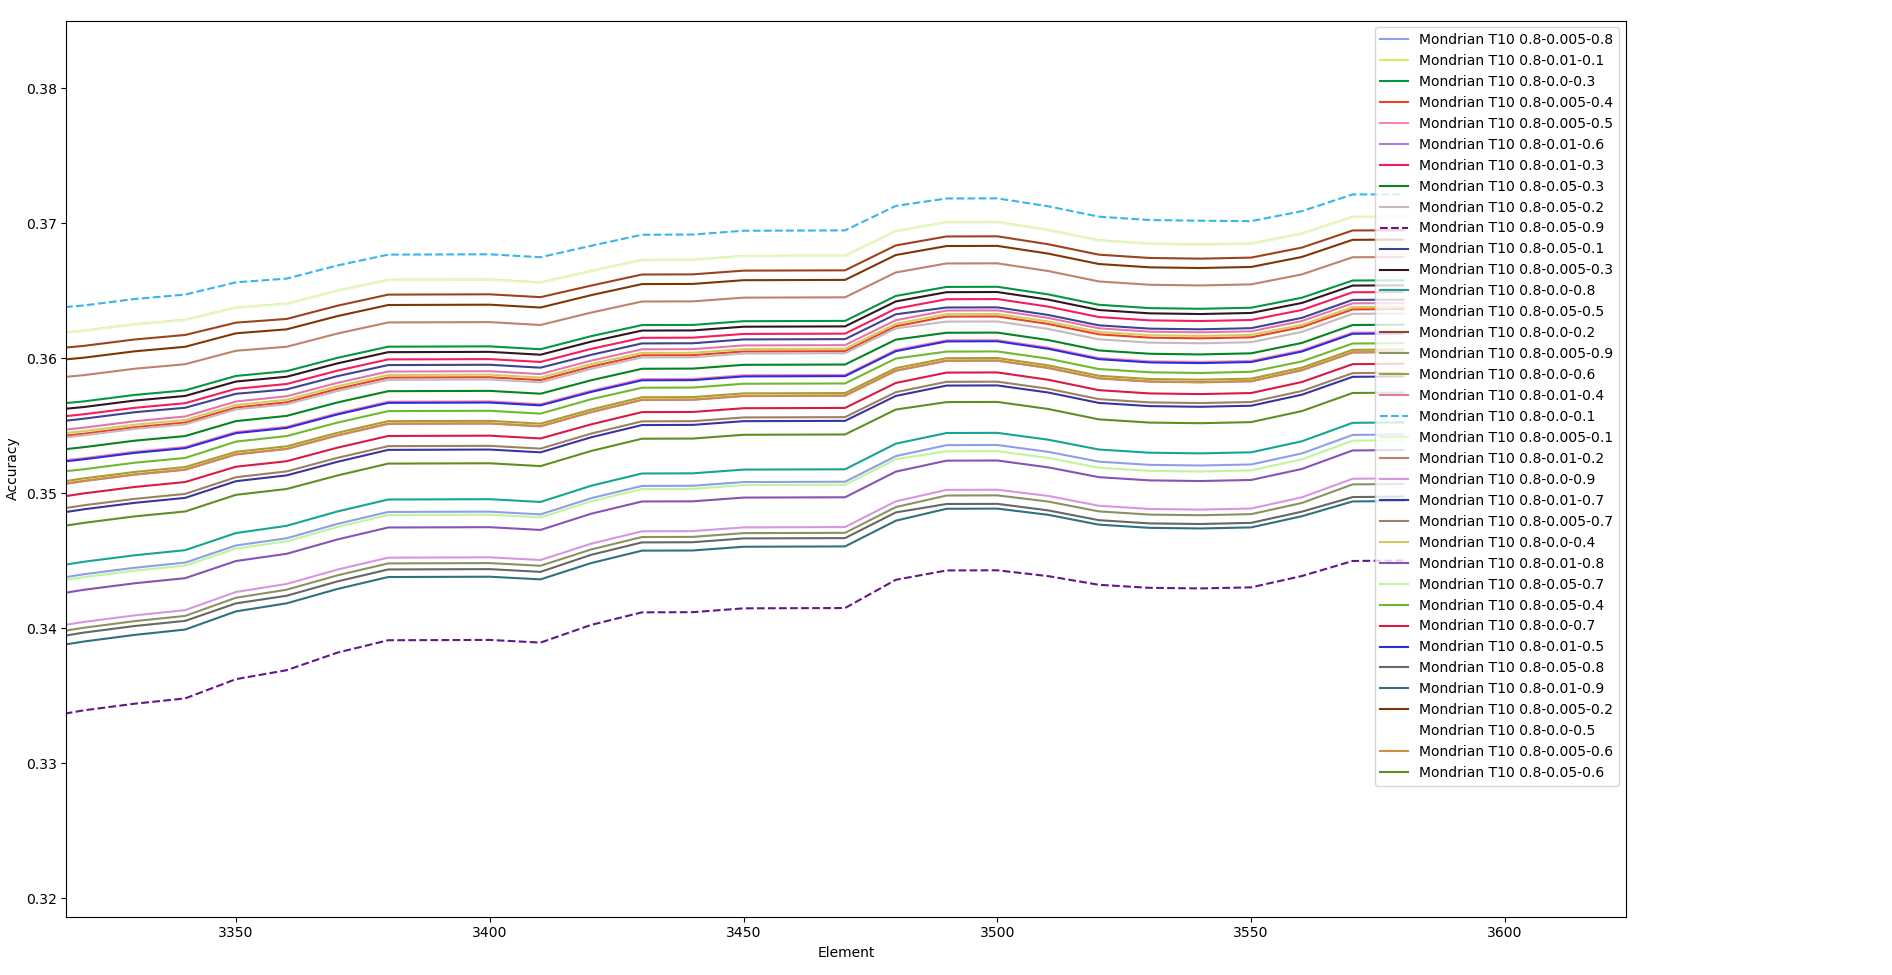
\includegraphics[width=\textwidth]{figures/Banos_S1_disount_check.png}
		 \caption{Impact of the discount factor with 10 trees, a budget of $1.0$, and a base count of $0.1$.}
		 \label{fig:mondrian-discount}
	 \end{subfigure}
		\caption{Mondrian tuning results.}
		\label{fig:mondrian-tuning}
\end{figure}


